%%%%%%%%%%%%%%%%%%%%%%%%%%%%%%%%%%%%%%%%%%%%%%%%%%%%%%%%%%%%%%%%%%%%%%
%%                                                                 %%
%% Please do not use \input{...} to include other tex files.       %%
%% Submit your LaTeX manuscript as one .tex document.              %%
%%                                                                 %%
%% All additional figures and files should be attached             %%
%% separately and not embedded in the \TeX\ document itself.       %%
%%                                                                 %%
%%%%%%%%%%%%%%%%%%%%%%%%%%%%%%%%%%%%%%%%%%%%%%%%%%%%%%%%%%%%%%%%%%%%%

\documentclass[sn-mathphys,Numbered]{sn-jnl}  % If you add `lineo` to have linenumbers here, you cannot skip linenumbering in tables

%%%% Standard Packages
%%<additional latex packages if required can be included here>
\usepackage{graphicx}%
\usepackage{multirow}%
\usepackage{amsmath,amssymb,amsfonts}%
\usepackage{amsthm}%
\usepackage{mathrsfs}%
\usepackage[title]{appendix}%
\usepackage{xcolor}%
\usepackage{textcomp}%
\usepackage{manyfoot}%
\usepackage{booktabs}%
\usepackage{algorithm}%
\usepackage{algorithmicx}%
\usepackage{algpseudocode}%
\usepackage{listings}%

%%%%
% REMOVE THOSE IN THE END
\usepackage{todonotes}
\usepackage{caption}
\usepackage{tabularx}
\usepackage{adjustbox}  % for the adjustwidth
\usepackage{threeparttable}  % to support notes within a table
\usepackage{makecell}  % For \makecell command

\usepackage{capt-of}


\renewcommand\theadfont{\bfseries}



%\jyear{2021}%

\theoremstyle{thmstyleone}%
\newtheorem{theorem}{Theorem}%  meant for continuous numbers
\newtheorem{proposition}[theorem]{Proposition}% 
\theoremstyle{thmstyletwo}%
\newtheorem{example}{Example}%
\newtheorem{remark}{Remark}%
\theoremstyle{thmstylethree}%
\newtheorem{definition}{Definition}%
\raggedbottom


\newcommand{\microbetag}{\texttt{microbetag }}

\usepackage{lineno}
\newenvironment{mytable}
{
    \nolinenumbers
    \begin{table}[ht]
    \centering
}
{
    \end{table}
    \linenumbers
}



\begin{document}

\linenumbers

\title[Article Title]{
    % Genomic, metabolic and literature oriented annotation of microbial co-occurrence networks enhances associations confidence level and hypothesis generation
    microbetag: simplifying microbial network interpretation through annotation, enrichment and metabolic complementarity analysis
}


%%==================================%%
%% Authors - affiliations           %%
%%==================================%%


\author[1]{\fnm{Haris} \sur{Zafeiropoulos}}\email{haris.zafeiropoulos@kuleuven.be}
\author[1]{\fnm{Ermis Ioannis} \sur{Michail Delopoulos}}\email{ermisioannis.michaildelopoulos@student.kuleuven.be}
\author[2]{\fnm{Andi} \sur{Erega}}\email{andi.erega@hest.ethz.ch}
\author[2]{\fnm{Annelies} \sur{Geirnaert}}\email{annelies.geirnaert@hest.ethz.ch}
\author[3]{\fnm{John} \sur{Morris}}\email{scooter@cgl.ucsf.edu}
\author*[1]{\fnm{Karoline} \sur{Faust}}\email{karoline.faust@kuleuven.be}


\affil*[1]{
    \orgdiv{
        Department of Microbiology, Immunology and Transplantation, Rega Institute for Medical Research
    }, 
    \orgname{KU Leuven}, 
    \orgaddress{
        \street{Herestraat}, \city{Leuven}, \postcode{3000}, \state{}, \country{Belgium}
    }
}

\affil[2]{
    \orgdiv{Institute of Food, Nutrition and Health}, 
    \orgname{ETH Zurich}, 
    \orgaddress{
        \street{Street}, \city{Zurich}, \postcode{8092}, \state{}, \country{Switzerland}
    }
}

\affil[3]{
    \orgdiv{Department of Pharmaceutical Chemistry}, 
    \orgname{University of California San Francisco}, 
    \orgaddress{
        \street{Street}, \city{San Francisco}, \postcode{94143}, \state{California}, \country{USA}
    }
}

%%==================================%%
%% unstructured abstract %%
%%==================================%%
\abstract{

    \footnote{
        Looks liks Chris Quince is~\href{https://microbiomejournal.biomedcentral.com/articles/sections/bioinformatics--algorithms-and-software}{our editor}.
    }

    Up to 350 words.

    The abstract must include the following separate sections:
    
    \textbf{Background:} the context and purpose of the study

    \textbf{Results:} the main findings

    \textbf{Conclusions:} a brief summary and potential implications


    \begin{figure}[H]
        \label{fig:abstract}
        \includegraphics[width=\columnwidth]{figs/figure_abstract.png}
        \caption*{
            Figure abstract. 
            
            % From a count table (bins or OTUs/ASVs) one can come up with a co-occurrence network. 
            % To better understand and assess the confidence level of these associations, microbetag annotates both taxa (nodes) 
            % and 
            % integrating 
            % genomic data 
            
        }
    \end{figure}

}
%%==================================%%
%% keywords                         %%
%%==================================%%
\keywords{
    microbial associations,
    enrichemnt analysis,
    data integration,
    pathway complementarity,
    seed set
}

\maketitle


%%==================================%%
%% MAIN BODY                        %%
%%==================================%%


% ====================================================
% Background
% ====================================================
% REMEMBER: To have a footnote in the \section{}, you need to have NO empty lines; otherwise latex will not compile
\section*{Background
\footnote{
We are to submit in the Microbiome journal as a "Software" manuscript, thus we follow~\href{https://microbiomejournal.biomedcentral.com/submission-guidelines/preparing-your-manuscript/software-article}{these rules}.
}
\footnote{
The Background section should explain the relevant context and the specific issue that the software described is intended to address.
No subheadings.
}
}
\label{sec:background}

    Microbial ecology plays a fundamental role in the stability and resilience of ecosystems and their processes; from soils, aquatic environments and biogeochemical cycles~\cite{yuan2021climate} to host-associated environments and the human health~\cite{raes2008molecular, faust2012microbialReviewInteractions}.
    Most microbial species live only in communities~\cite{rottjers2018hairballs} and most natural microbial communities consist of hundreds or even thousands of species~\cite{balint2016millions}.
    Each species exhibits a unique repertoire of reactions and adapts to various niches, each with specific nutrient and environmental requirements.
    % KF: "To unravel microbial ecology involves disentangling the principles that dictate the organization of a community"... sounds rather pompous, can you tone it down a bit? we don't really look at the principles of community organisation in this work.
    % HZ: What about now ?
    Understanding the dynamics governing interactions among microbial species and their relationships with the surrounding environment would shed light in several aspects microbial ecology~\cite{robinson2010structure}.
    % references if we'd like to talk about microb com as ~\textit{complex systems}: ~\cite{godfray1990complex, amor2017spatial},

    % KF: what is the link of all this to microbetag? I suggest to strongly reduce this part
    % HZ: I remove the paragraph regarding the taxonomic vs functional variability; I had an idea on that but it would get too long to get there.. 
    %       For the paper we were discussing reg. an analysis on microbetagDB data this might be a nice question to ask! :)    
    % KF: and write instead more about:
    %        interaction mechanisms and 
    %        why it is so difficult to infer interactions from abundance data
    Based on the net fitness effects that result for the taxa involved, the notion of an interaction varies including cooperation, competition, parasitism, commensalism and ammensalism~\cite{faust2012microbialReviewInteractions}.
    Metabolic interactions can be established through a range of contact-independent- and contact-dependent mechanisms leading to both positive and negative interactions. 
    These interactions can involve either one-way (unidirectional) or two-way (bidirectional) exchanges of metabolites.
    Depending on the biosynthetic cost borne by the interacting partners, two types of metabolite exchanges occur: by-product cross-feeding, where metabolites result from a selfish act of the producer, and cooperative cross-feeding, where one partner actively invests resources to produce metabolites benefiting the interaction partner~\cite{d2018ecology}.


    High-throughput sequencing (HTS) has provided great insight into the diversity and composition of microbial communities~\cite{elixir_microbiome}. % get more refs
    Uncultivated species can now be detected, and their features can be inferred through their genomic information~\cite{hug2016new}.
    Moreover, the composition of thousands of microbiome samples is now accessible allowing for the inference of patterns among sets of samples.
    A widely used approach to extract such patterns, is the creation of co-occurrence networks based on metagenomic read data (amplicon and/or shotgun)~\cite{matchado2021network}. 
    A great number of approaches is available for co-occurrence network inference based on a range of statistical concepts such as: correlation (e.g., CoNet~\cite{faust2012microbial}, SparCC~\cite{friedman2012inferring}), linear regression (e.g., SpiecEasi~\cite{kurtz2015sparse}) and causal inference (FlashWeave~\cite{flashweave_cite}).
    Nevertheless, microbial co-occurrence networks continue to encounter various challenges~\cite{faust2021open}.
    Their inference inherits the challenges of metagenomic data analysis (e.g., compositionality, parameters inference)~\cite{cao2017inferring}.
    As a result, network construction remains a tool-dependent analysis~\cite{kishore2023inferring, weiss2016correlation}.
    Moreover, more often than not, the returned network looks like a "hairball" of densely interconnected taxa.
    Thus, additional analysis is necessary to generate testable hypotheses~\cite{faust2021open}.
    Addressing the question of~\textit{What can we learn from the hairballs} posed by R{\"o}ttjers et \textit{al.}~\cite{rottjers2018hairballs} could provide essential insight on the mechanisms of the interactions.

    % KF: why has the use of network inference for interaction prediction underscored its limited accuracy? Imprecise expression: the use itself did not underscore the low accuracy - evaluations did. This needs to be rephrased.
    % HZ: How about now ?
    The assessment of interaction predictions derived from microbial co-occurrence networks has underscored their limitations in accuracy for this task~\cite{berry2014deciphering}.
    Theoretical principles derived from network studies might provide indications of emergent biological characteristics~\cite{rottjers2018hairballs, guo2022microbial}. 
    For example, modules (highly interconnected nodes) within microbial co-occurrence networks could serve as indicators of ecological processes that govern community structure, including niche filtering and habitat preference~\cite{ma2020earth}.
    Data integration and clustering have been suggested to address this challenge~\cite{faust2021open}.
    Clusters identified in microbial association networks have demonstrated their ability to mirror key drivers of community composition~\cite{guidi2016plankton} and several algorithms and implementations are available~\cite{rottjers2020manta}.
    However, data integration approaches in microbial co-occurrence networks are so-far limited.
    Here, we present \microbetag, a microbial co-occurrence network annotator that exploits several channels of information to enhance/diminish the confidence of the associations suggested by the network and generate hypotheses for further investigation both at the taxon pair and the community level.

    \microbetag serves as a comprehensive platform that provides information on taxa along with their potential metabolic interactions from multiple channels 
    (see Implementation~\ref{sec:implementation}).
    % literature-based classification of OTUs and their corresponding taxonomies to functional groups, 
    % prediction of microbial phenotypes via comparative genomics
    The key concept here is the reverse ecology approach~\textit{reverse ecology}~\cite{levy2012reverse}.
    Reverse ecology leverages genomics to explore community ecology with no \textit{a priori} assumptions about the taxa involved.
    Making the most of the advancements in systems biology and genomic metabolic modeling, as well as system-level analysis of intricate biological networks, the reverse ecology framework enables the prediction of ecological traits for less-understood microorganisms, their interactions with others, and the overall ecology of microbial communities~\cite{levy2014metagenomic}.
    % KF: what was major about the seed set analysis? Did we learn anything useful from it so far? I don't think so, so please tone it down.
    % HZ: I suggest we just remove this. 
    % In this context, seed set analysis has been a major contribution in the study of both the species and the community ecology based on their genetic information.

    A metabolic network's "seed set" is the set of compounds that, based on the network topology, need to be acquired exogenously~\cite{borenstein2008large}~(see Figure~\ref{fig:pathcompl}).
    Such nodes might be independent, i.e. they cannot be activated by any other node in the network, or they can be interdependent forming groups of seed nodes.
    Seeds are a useful proxy for the habitat of the organism and an essential tool in the framework of reverse ecology~\cite{parter2007environmental,borenstein2008large}.
    Based on the seed concept, several graph theory-based metrics (indices) have been described to predict species interactions directly from their networks' topologies~\cite{levy2015netcooperate, kreimer2012netcmpt, zelezniak2015metabolic, belcour2020metage2metabo}.
    Over the last years, the seed approach has been implemented at the Genome-scale metabolic network reconstructions (GENREs) level.
    GENREs encapsulate mathematical representations capturing the biochemical reactions that could take place within an organism~\cite{thiele2010protocol, durot2008genome, communityGemMicrobiomeModel2023}.

    Metabolic complementarity among species, serving as a reflection of potential cooperation within communities, assesses the capacity for collaboration; cross-feeding or syntrophy interactions are typical examples of such a collaboration. 
    In contrast, metabolic competition refers to the metabolic overlap between two species leading to exploitative competition, e.g. for nutrient resources.
    Seed and non-seed sets can be used to compute such indices. 
    Thorough examination of such complements can reveal metabolic interactions leading to patterns observed on the co-occurrence network.
    
    % KF: In addition, I don't get the meaning of the first part of this sentence
    % HZ: How about now ?
    However, Bacteria may complement each other not only for getting what is absolutely necessary for them to survive (seeds).
    For example, microbial species are recognized to exchange metabolites in order to provide support for other advantageous services, such as detoxifying harmful metabolites or offering protection against predators~\cite{little2008rules, zientz2004metabolic}.
    They can additionally contribute to the production of metabolites essential for the entire community, even if the species itself does not require them~\cite{kallus2017paradoxes}.
    To explore the potential of a species metabolism given they benefit from a partner of theirs, genome annotations combined with collections of functional units to highlight can provide a valid proxy.
    We present here a naive approach exporting all possible complements between a pair of species based on their KEGG ORTHOLOGY (KOs) annotations and the KEGG MODULES database~\cite{keggmodulesdb}.

    \microbetag annotates a user's co-occurrence network by integrating phenotypic traits on the taxa present on the network (nodes) and potential metabolic interactions to their suggested associations (edges).
    A Graphical User Interface (GUI) is supported as a CytoscapeApp providing a user-friendly environment to investigate annotations in a straightforward way.
    All annotations present in microbetagDB are also available through an Application Programming Interface (API).
    \microbetag's source code is distributed under a GNU GPL v3 license and available on GitHub. 
    Documentation and further support on how to use \microbetag is available at \href{https://hariszaf.github.io/microbetag/}{documentation web-site}.
    To the best of our knowledge there is not a software with which \microbetag could be compared with directly. 
    To validate our annotations we used a recently published network with partially known interactions between some pairs of species found associated~\cite{hessler2023vitamin} (see Results section, paragraph~\ref{subsec:validation}).    
    To demonstrate \microbetag's potential, we present the main features of its interface, and we discuss a real-world use-case (see Discussion section, paragraph~\ref{subsec:usecase}).


    % ===================           for easy access to some nice parts         =====================

    % ~~~~~~~~~~~~~~~~~~
    % In recent years, there has been a compelling suggestion proposing an elegant paradigm for microbial ecology: 
    %the correlation between community functional and taxonomic composition depends on the relative importance of metabolic niche effects 
    %% (influence of specific metabolic conditions and requirements within an environment on the composition and distribution of microbial functions)
    %compared to processes causing variation within functional groups 
    %% (genetic diversity, regulatory mechanisms, environmental influences, and stochastic events affecting individual members of the functional group)

    % (rephrased)
    % Metabolic conditions within an environment influence the composition and distribution of its functions (metabolic niche effect).
    % At the same time, processes like genetic diversity and stochastic events, induce variability within different functional groups of the community.
    % Recent studies suggest that the relative importance of those two processes drive the extent to which functional and taxonomic composition at the community level are correlated~\cite{louca2016high}.
    % ~~~~~~~~~~~~~~~~~~

    % % ----------   Taxonomy - functional composiiton relationship ---------------
    % In this case, comparable environments should foster similar microbial community functions, even though there may be taxonomic variations within individual functional groups, 
    % while in more heterogeneous environments functional $\beta$ diversity would be strongly correlated with taxonomic $\beta$ diversity.
    % In the latter, the decoupling between community composition and metabolic functioning is concealed by robust metabolic niche effect~\cite{louca2016high}.
    % Thus, an interaction between two taxa may vary in different environments.
    % Microbial interactions can be the result of multiple phenomena, such as exchange of metabolic products~\cite{kost2023metabolic}, biofilm formation~\cite{arnaouteli2021bacillus}, gene transfering~\cite{de2023horizontal} and signaling~\cite{keller2006communication}.
    % % The metabolic function of a community undergoes substantial influence from energetic and stoichiometric constraints~\cite{george2023functional}.

    % From~\cite{louca2016high}
    % Ecological communities are governed by an interplay of deterministic processes associated with species interactions with their environment (environmental filtering) and each other (limiting similarity)1,2.

    % the metabolic functional potential of microbial communities in the global ocean or in soil is closely related to environmental conditions, while the taxonomic variation within individual functional groups is only poorly explained by environmental condition

    % community metabolic function is strongly shaped by energetic and stoichiometric constraints such as the availability of electron acceptors for respiration10, while the composition within functional groups is modulated by additional mechanisms.

    % According to this paradigm, \textbf{similar environments should promote similar microbial community function, while allowing for taxonomic variation within individual functional groups}.

    % These interactions contribute to the overall stability and functioning of ecosystems by influencing nutrient cycling, disease dynamics, and the overall diversity and composition of microbial communities. 
    % For example, some microorganisms can produce and release certain compounds that benefit neighboring microbes or inhibit the growth of competing species. 
    % Other interactions involve symbiotic relationships, where different microbes rely on each other for survival and perform complementary functions. 
    % Understanding and studying microbial interactions is vital for unraveling the complexity of microbial communities and their impact on human health, agriculture, and environmental processes.

    % metabolic interactions specifically, microorganisms often engage in metabolic exchanges during their interactions. 
    % For instance, one microbe may produce metabolites that serve as nutrients or signaling molecules for another microbe. These metabolic interactions can involve the transfer of essential nutrients, the breakdown of complex compounds, or the production of secondary metabolites with antimicrobial properties.
    % Overall, understanding the different types of microbial interactions, including metabolic interactions, provides insights into the complexity and dynamics of microbial communities and their impact on various processes in nature.


 
% ====================================================
% Implementation
% ====================================================
\section*{Implementation
    \footnote{
        This should include a description of the overall architecture of the software implementation, along with details of any critical issues and how they were addressed.
    }
}
\label{sec:implementation}


    % ---------------------
    % FIGURE for precalculations (fig:precalc)
    % ---------------------
    \begin{figure}[h!]
        \label{fig:precalc}
        \includegraphics[width=0.9\columnwidth]{figs/microbetag-precal.png}
        \caption{
            Diagram of the \microbetag pre - calculations (top panel) and the on the fly workflow (bottom panel). 
            GTDB v207 representative genomes were filtered and for those of high-quality
            33 phenotypic traits were predicted using~\texttt{phenotrex}.
            To this end, models were re-trained to sync with recent version of eggNOG.
        }
    \end{figure}


    \subsection*{Genomes included}
    \label{subsec:genomes}

        Using the Genome Taxonomy Database (GTDB) v207 \href{https://data.gtdb.ecogenomic.org/releases/release207/207.0/}{metadata files}, we retrieved the NCBI genome accessions of the high quality representative genomes, i.e. completeness $\geq 95\%$  and contamination $\leq 5\%$.
        % That resulted a set of $26,778$ covering $22,009$ unique NCBI Taxonomy Ids.
        A set of $26,778$ genomes was obtained, representing $22,009$ unique NCBI Taxonomy Ids.
        Using these accession numbers, we were able to download their corresponding \texttt{.faa} files when available 
        % (\href{https://github.com/hariszaf/microbetag/blob/develop/microbetagDB/mappings/gtdb_ncbi/get_gtdb_faa.py}{\texttt{get\_gtdb\_faa.py}}) 
        leading to a set of $16,900$ amino acid sequence files.
        The latter were annotated and used to obtain potential pathway complementarities between pairs of genomes (see paragraph~\ref{subsec:path-compl}).
        Last, when available, their corresponding annotations on PATRIC database~\cite{wattam2017improvements} were retrieved to reconstruct GENREs~(see paragraph~\ref{subsec:seeds}).


    \subsection*{Taxonomy schemes}
    \label{subsec:taxonomies}

        \microbetag maps the taxonomy of each entry in the abundance table to their corresponding NCBI Taxonomy Id and, if available, their closest GTDB representative genome(s), since several GTDB representative genomes may map to the same NCBI Taxonomy Id.
        Two well established taxonomy schemes are supported: the GTDB~\cite{parks2022gtdb} that is being broadly used for bins and/or MAGs taxonomic classification and the Silva database~\cite{quast2012silva} that is widely used in amplicon studies. Both taxonomy schemes link their taxonomies to NCBI Taxonomy Ids~\cite{schoch2020ncbi}.
        In case none of those two taxonomies was used, and the abundance table contains less than 1,000 taxa, \microbetag maps the user provided taxonomies to NCBI Taxonomy. 
        %However, this is done only for abundance tables containing less the 1,000 taxa. 
        To this end, \microbetag makes use of the~\href{https://github.com/seatgeek/thefuzz}{\texttt{fuzzywuzzy}} library that implements the Levenshtein Distance Metric to get the closest NCBI taxon name and thus its corresponding NCBI Taxonomy Id; a relatively high similarity score is used (90) to avoid false positives. 
        Also, using the nodes dump file of NCBI Taxonomy, \microbetag may retrieve the child taxa of a taxon in user's data, along with their corresponding NCBI Taxonomy Ids, if requested by the user.
        % Thus, \microbetag maps a network taxon to their corresponding NCBI Taxonomy Id and if available their corresponding GTDB genomes.
        If the user provides their abundance table with taxonomies already mapped to the GTDB taxonomy, \microbetag will report the best possible annotations in a time efficient manner. 
        % as it is both time efficient and, mainly, it allows for the best annotations \microbetag could report, it is strongly suggested that both amplicon and shotgun-oriented data to be mapped to GTDB taxonomies.
        
        % Having a taxonomy scheme of GTDB or Silva is mandatory for networks with more than $1,000$ taxa.
        
        % The corresponding taxonomy will be mentioned as "microbetag\_prep".
        
        % There is a great number of taxonomies that are being used in such studies, e.g. Silva~\cite{quast2012silva}, Ribosomal Database Project (RDP)~\cite{cole2014ribosomal}, manually curated ones and more, 
        % As a consequence, there is not a standardised format of the taxonomies assigned, from bioinformatics pipelines used for the analysis of such data.


    \subsection*{Network inference}
    \label{subsec:net-infer}

        When a co-occurrence network is not provided by the user, \microbetag exploits FlashWeave~\cite{flashweave_cite} to build one on the fly.
        Yet, \microbetag supports the annotation of networks built from any algorithm/software, in any format Cytoscape can load.

        % a computational approach based on a flexible Probabilistic Graphical Model framework that integrates metadata and predicts direct microbial interactions from heterogeneous microbial abundance data sets with hundreds of thousands of samples. 
        % A flexible Probabilistic Graphical Model framework is used in a computational approach that 
        % incorporates metadata and predicts direct microbial interactions. 
        % This is done using heterogeneous microbial abundance datasets consisting of hundreds of thousands of samples.

        %     •    heterogeneous - enable heterogeneous mode for multi-habitat or -protocol data with at least thousands of samples (FlashWeaveHE)
        %     •    sensitive - enable fine-grained associations (FlashWeave-S, FlashWeaveHE-S), sensitive=false results in the fast modes FlashWeave-F or FlashWeaveHE-F
        %     •    FDR - perform False Discovery Rate correction (Benjamini-Hochberg method) on pairwise associations
        %     •    n_obs_min - don't compute associations between variables having less reliable samples (i.e. non-zero if heterogeneous=true) than this number. -1: automatically choose a threshold.

    \subsection*{\microbetag pre-processing}
    \label{subsec:preprocess}

        In order to aid the user to map their sequences to the GTDB taxonomy, DADA2-formatted 16S rRNA gene sequences for both bacteria and archaea~\cite{ali_alishum_2022_6655692} were used to train the IDTAXA classifier of the DECIPHER package~\cite{{murali2018idtaxa}} and are available through the~\href{https:/hub.docker.com/repository/docker/hariszaf/microbetag_prep/}{microbetag preprocess Docker image}.
        Likewise, when the abundance table consists of more than $1,000$ taxa, providing a network as an input is mandatory.
        Again, to help the user, \microbetag preprocess Docker image supports the inference of a network using FlashWeave.

        For a computationally efficient way to annotate large networks, a Docker image is provided, so the user runs a taxonomy assignment using the IDTAXA algorithm~\cite{murali2018idtaxa} of the DECIPHER R package~\cite{wright2016using}.
        A co-occurrence network is also built using FlashWeave~\cite{flashweave_cite}, as \microbetag also does.


    \subsection*{Literature based nodes annotation}
    \label{subsec:fapro}

        Using a set of Tara Ocean samples~\cite{sunagawa2015structure} FAPROTAX~\cite{louca2016decoupling} estimates the functional potential of the bacterial and archaeal communities, by classifying each taxonomic unit into functional group(s) based on current literature, descriptions of cultured representatives and/or manuals of systematic microbiology. 
        In this manually curated approach, a taxon is associated with a function if and only if all the cultured species within the taxon have been shown to exhibit that function. 
        % Apparently, FAPROTAX does not support the annotation of clades with no cultured representatives that have been rising thanks to high throughput sequencing technologies.
        % Further, a taxon could be annotated with more than one functions while functional groups could be nested.
        In its current version, FAPROTAX includes more than 80 functions based on ~7600 functional annotations and covering more than 4600 taxa.
        Contrary to gene content based approaches, e.g. PICRUSt2~\cite{douglas2020picrust2}, FAPROTAX  estimates metabolic phenotypes based on experimental evidence. 

        \microbetag invokes the accompanying script of FAPROTAX and converts the taxonomic microbial community profile of the samples included in the user's abundance table or of the taxa present in the provided network, into putative functional profiles.
        Then, it parses FAPROTAX's sub-tables to annotate each taxonomic unit present in the user's data with all the functions for which they had a hit. 
        FAPROTAX annotations are not part of the microbetagDB but are computed on the fly.


    \subsection*{Genomic based nodes annotation}
    \label{subsec:phen}

        phenDB~\cite{feldbauer2015prediction} is a publicly available resource that supports the analysis of bacterial (meta)genomes to identify 47 distinct functional traits, e.g. whether a species is producing butanol or has a halophilic lifestyle.
        It relies on support vector machines (SVM) trained with manually curated datasets based on gene presence/absence patterns for trait prediction.
        More specifically, the model for a particular trait is trained using a collection of EggNOG annotated genomes where the knowledge of whether that trait is present or absent among its members is available.
        These models (classifiers) are used to predict presence/absence of their corresponding traits in non-studied species. 
        % Based on the completeness/contamination of the genomes, the accuracy varies. 
        % The~\texttt{compute-genotype} program of phenotrex supports the creation of such tabular~\textit{genotype} files.
        % A~\textit{genotype} file can be used along with a~\textit{phenotype} one, i.e., a file containing true phenotypic trait values for each input genome on which to train the model, and the~\texttt{train} program of phenotrex can then be performed. 

        % one can implement tests to evaluate the model based on the completeness of a genomes and its contamination (Performance Estimation) using the cccv program. e.g
        % {
        % 	"mean_balanced_accuracy": 0.5499999999999999,
        % 	"stddev_balanced_accuracy": 0.10482201257840669,
        % 	"contamination": 0.7,
        % 	"completeness": 1.0
        % },
        In the framework of microbetagDB, %phenotrex 
        classifiers were re-trained using the genomes provided by phenDB for each trait to sync with the latest version of eggNOG~\cite{huerta2019eggnog} and the~\texttt{phenotrex}~\cite{feldbauer2015prediction} software tool.
        Genomes were downloaded from NCBI using the \href{https://www.ncbi.nlm.nih.gov/sites/batchentrez}{Batch Entrez} program.
        % as there was a conflict between the eggNOG version phenotrex uses at the prediction step and the one during the training of the classes as provided in the PhenDB site.
        % For example, for the acetic acid production case, the corresponding webpage of phenDB pointed to the set of genomes that had been originally used. 
        Then, \textit{genotype} files were produced for all the high quality GTDB representative genomes.
        Each model was then used against all the GTDB \textit{genotype} files to annotate each with the presence or the absence of the trait. 
        A list of all the phenotypic traits available for the genomes present in microbetagDB is available on \microbetag 's \href{https://hariszaf.github.io/microbetag/docs/modules/phen-traits/}{documentation site}.
        The updated models are also available


    \subsection*{Pathway complementarity}
    \label{subsec:path-compl}


        To infer potential pathway complementarities we consider the modules described in KEGG MODULES database~\cite{keggmodulesdb}.
        % as functional units to highlight can provide a valid proxy.
        A KEGG module is defined as a functional unit within the KEGG framework that represents a set of enzymes and reactions involved in a specific biological process or pathway~\cite{muto2013modular}.
        Such a unit consists of several~\textit{steps}, each of which may have more than one molecular ways to occur (Figure~\ref{fig:pathcompl}).
        A module's definition is a logical expression and consists of KOs 
        % and the following symbols:
        that may be coupled with one another as:
            % a. the space, representing a connection in the pathway
            a. connected steps of the pathway
            % b. plus sign, representing a molecular complex,
            b. parts of a molecular complex, 
            % c. comma, representing alternatives and
            c. alternatives of the same step, and 
            % d. minus sign, designates an optional item in the complex.
            d. optional entities of a complex.
        Both (a) and (b) cases should be considered as the~\texttt{AND} logical operator, while (c) would be the~\texttt{OR} (Figure~\ref{fig:pathcompl}).
        Given a module's definition, we will consider as an~\textit{alternative} any subset of the KO terms mentioned in the definition, 
        that has exactly one way to perform each step, provided that all the steps of the module are covered.
        % and support the functioning of all the steps of the module.
        We define a genome as having a~\textit{complete} module, if and only if all the KOs of at least one alternative are present on the genome.
        In Appendix~\ref{app:pathcompl} we show an example of a module along with its alternatives.

        Within this framework,~\texttt{kofamscan}~\cite{aramaki2020kofamkoala} was used to annotate with KEGG ORTHOLOGY terms (KOs) the $16,900$ high quality GTDB representative genomes for which a~\texttt{.faa} was available~\cite{kanehisa2012kegg}.
        The KOs of each genome were then mapped to their corresponding KEGG modules; a KO may map to more than one module ($1:n$).
        % , see Appendix~\ref{secA2}).

        \begin{figure}[h!]
            \includegraphics*[width=0.8\columnwidth]{figs/path_complem.png}
            \caption{
                Pathway complementarity approach. 
                The high quality GTDB genomes were annotated with KEGG ORTHOLOGY (KO) terms.
                The various ways of getting a KEGG module complete were enumerated and all the possible ways a donor species could "fill" a beneficiary's non-complete module were calculated.
                In this case, there are 4 unique ways for having the serine biosynthesis module complete; in all of them K00831 is required.
                However, it is missing from the beneficiary species that supports the 2 out of the 3 steps of the module's definition.
                A donor species having and potentially sharing the corresponding enzyme of K00831 may enable the beneficiary species to produce serine.
            }
            \label{fig:pathcompl}
        \end{figure}

        All module definitions were retrieved using the KEGG API and parsed to enumerate their alternatives.
        % (\href{https://github.com/hariszaf/microbetag/blob/develop/microbetagDB/mappings/kegg_mappings/parse_module_definitions.py}{\texttt{parse\_module\_definitions.py}}).
        % A dictionary was built with all the alternatives of each module. 
        %, i.e. alternative sets of KOs, for a module to be complete.
        % (\href{https://github.com/hariszaf/microbetag/blob/develop/microbetagDB/mappings/kegg_mappings/module_definition_map.json}{module\_definition\_map.json})
        Each pair of the KEGG annotated genomes was then investigated for potential pathway complementarities, 
        i.e. whether a genome lacking a number of KOs ($genome_A$) to have a complete module ($module_x$) could benefit from another's species genome(s) ($genome_B$).
        In that case, $genome_B$ does not necessarily have a complete alternative of $module_x$; as long as it has the missing KOs that $genome_A$ needs to complete an alternative of it, $genome_B$ potentially complements $genome_A$ with respect to $module_x$.
        In total, $341,568$ unique complementarities were exported.
        % (\href{https://github.com/hariszaf/microbetag/blob/develop/microbetagDB/scripts/pathway_complementarity.py}{\texttt{pathway\_complementarity.py}})

        Thanks to the graphical user interface (GUI) of the~\href{https://www.kegg.jp/kegg/docs/color_gui.html}{KEGG pathway map viewer}~\cite{kanehisa2020kegg,kanehisa2022kegg}, 
        each complementarity can be visualised as part of the closest KEGG metabolic map; 
        where the KOs contributed by the donor are shown in blue-green whereas those coming from the beneficiary genome are coloured in red.

        \microbetag annotates the edges of a co-occurrence network by identifying pairs where both taxa map to an annotated genome present on microbetagDB.
        % Each taxon on the network has been mapped to a NCBI Taxonomy Id and their related GTDB genomes.
        Since co-occurrence networks are undirected, both nodes of a suggested association are considered as potential donors and beneficiary species. 
        When more than one GTDB representative genome map to the same NCBI Taxonomy Id all the possible genome combinations are considered.
        Finally, two edges are added in such pairs of taxa in the annotated network: 
        one considering $species_A$ as the potential beneficiary and $species_B$ as the potential donor species, and one vice-versa. 


    \subsection*{Seed scores and complements using genome scale metabolic reconstructions }
    \label{subsec:seeds}

        The Metabolic Complementarity Index ($MI_{Complementarity}$) measures the degree to which two microbial species can mutually assist each other by complementing each other's biosynthetic capabilities.
        As described in~\cite{phylomint_ms}, it is defined as the proportion of seed compounds of a species that can be synthesized by the metabolic network of another, but are not included in the seed set of the latter. 
        $MI_{Complementarity}$ offers an upper bound assessment of the potential for syntrophic interactions between two species.
        Further, the Metabolic Competition Index ($MI_{Competition}$) represents the similarity in two species' nutritional profiles. 
        This index establishes an upper limit on the level of competition that one species may face from another.
        Those indices have been thoroughly described and implemented in the NetCooperate~\cite{levy2015netcooperate} and NetCompt~\cite{kreimer2012netcmpt} tools correspondingly.
        We will be referring to those two indices as "seed scores".
        Recently, the~\texttt{PhyloMint} tool~\cite{phylomint_ms} was released supporting the calculation of the seed scores of GENREs in SBML format.

        In the~\microbetag framework, seed scores were computed using GENREs derived from the high quality GTDB representative genomes and the~\texttt{PhyloMint} tool.
        GENREs were reconstructed using the Model SEED pipeline~\cite{henry2010high} through its Python interface \href{https://modelseedpy.readthedocs.io/en/latest/index.html}{ModelSEEDpy}.
        The latter requires RAST annotated genomes~\cite{overbeek2014seed}; 
        if available through the PATRIC database~\cite{wattam2017improvements}, annotations were retrieved.
        For the rest of the genomes, RAST annotation was performed through RASTtk~\cite{brettin2015rasttk}.

        Moreover, the computed seed and the non-seed (i.e., set of metabolic compounds a genome can build on its own) sets of each genome were used to compute their overlap among all the pairwise combinations of those genomes.
        More specifically, seed and non-seed compounds of each genome were mapped to their corresponding KO terms and those related to any KEGG MODULE were considered.
        The latter were then used for the calculation of the overlap of ${seed\ set}_{species_A}$ with the ${non\ seed\ set}_{species_B}$ was retrieved.
        \microbetag then annotates again the edges of the co-occurrence network where both taxa have been mapped to a at least one GTDB genome, mentioning all the KEGG maps for which there is at least one seed compound of the potentially beneficiary species 



    \subsection*{Clustering network}
    \label{subsec:manta}

        % KF: sentence not complete
        \texttt{manta} is a heuristic network clustering algorithm that clusters nodes within weighted networks effectively, leveraging the presence of negative edges and discerning between weak and strong cluster assignments.
        \microbetag invokes manta~\cite{rottjers2020manta} to infer clusters from the microbial network.
        In case \texttt{manta} is performed, the annotated network inherits the layout that \texttt{manta} returns.


    \subsection*{The~\microbetag workflow}
    \label{subsec:app}
        % --------------------
        % FIGURE for workflow overall (fig:wf)
        % --------------------
        \begin{figure}[h!]
            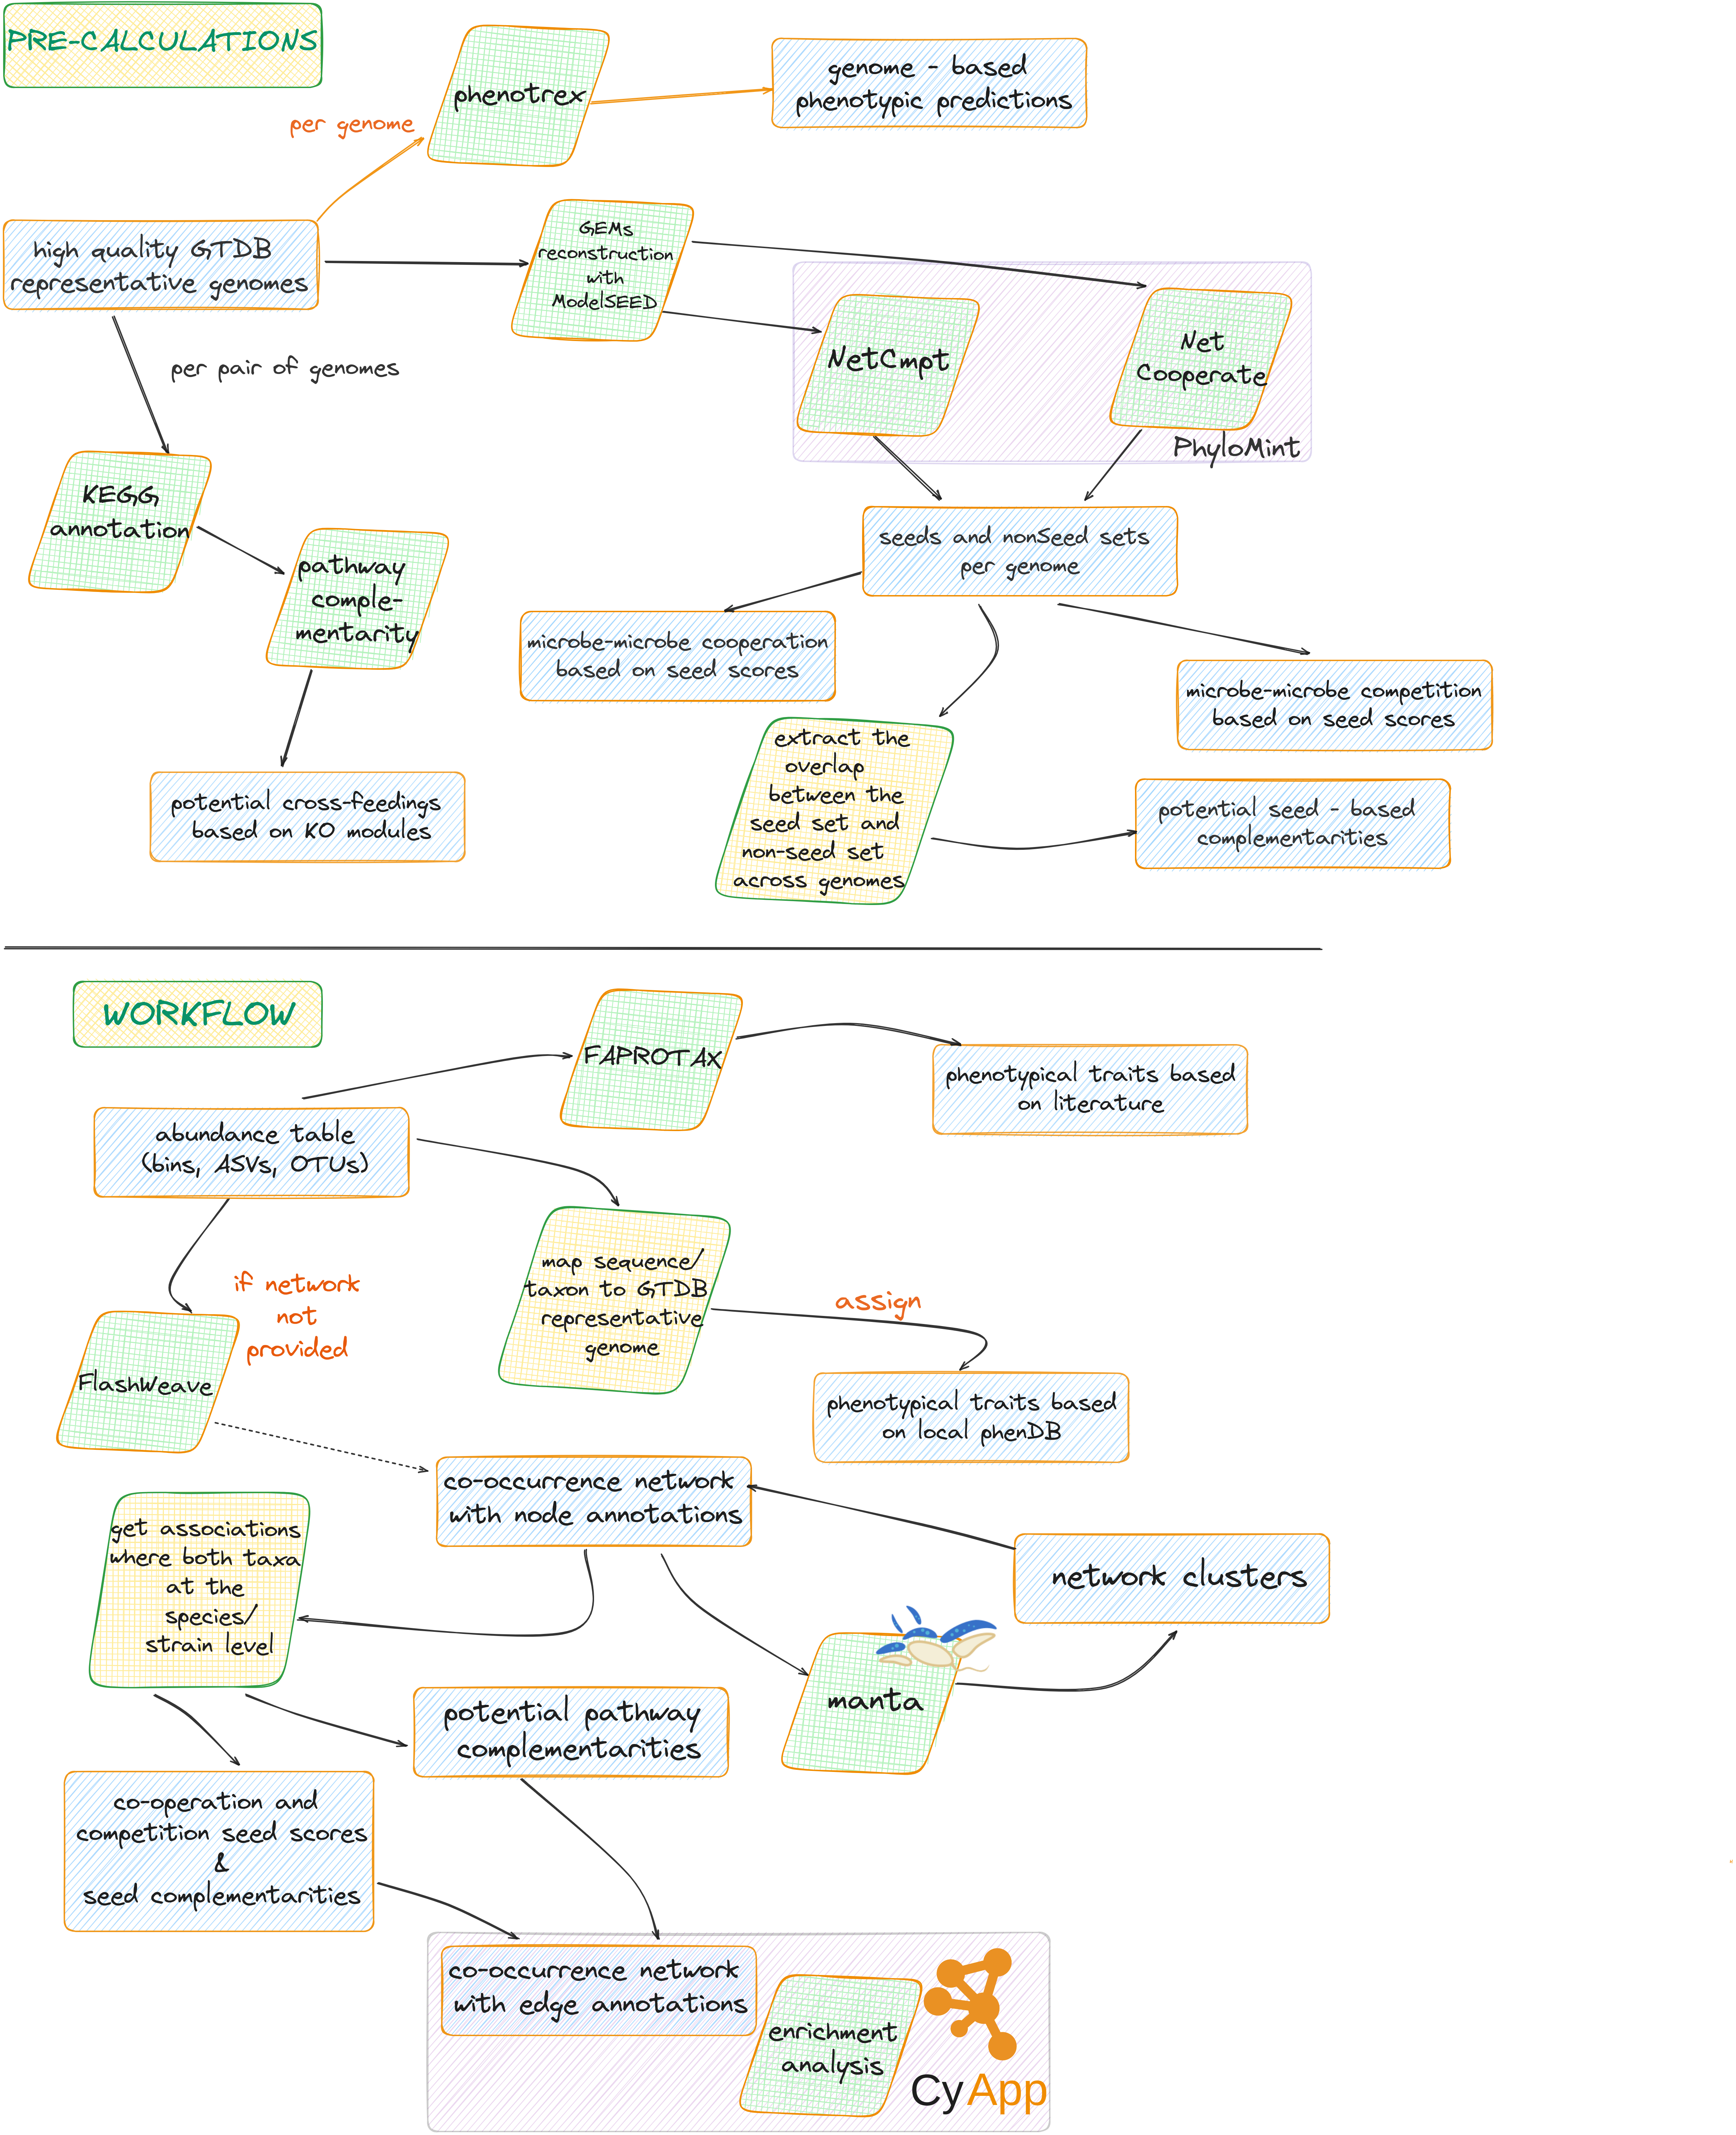
\includegraphics[width=0.9\columnwidth]{figs/microbetag-wf.png}
            \caption{
                Diagram of \microbetag's on-the-fly workflow. 
                \microbetag expects either an abundance table only as input and infers a co-occurrence network using FlashWeave 
                or an abundance table along with an already inferred co-occurrence network 
                and after mapping taxa present to GTDB reference genomes, for those possible, phenotypic attributes are assigned on the nodes. 
                Literature-based annotation on the nodes are also using FAPROTAX.
                On the edges level then, \microbetag annotates them by assigning the pre-calculated potential complements based on the pathway and the seed complementarities approaches. 
                \microbetag supports optional network clustering with manta.
                The annotated network can then be parsed on Cytoscape using the MGG app.
            }
            \label{fig:wf}
        \end{figure}


        As shown in Figure~\ref{fig:wf}, the~\microbetag workflow expects an abundance table representing either amplicon or shotgun data.
        If a co-occurrence network is already available the user may provide it too as input.
        The~\microbetag workflow will first map the taxa present on the abundance table to their corresponding GTDB representative genomes if that is possible, i.e., in case the taxonomy provided does reach the species or the strain level (see paragraph~\ref{subsec:taxonomies}).
        If a network is not provided, \microbetag will then build one using FlashWeave~\cite{flashweave_cite}. 
        Then the abundance table will be used for a literature - based annotation using FAPROTAX~\cite{louca2016decoupling}.
        This is the only annotation step that is microbetagDB independent in the framework of the web-service workflow.
        The nodes of the network will be further annotated with phenotypic traits based on the model predictions~\cite{feldbauer2015prediction}.
        Edges linking taxa that have been assigned to the species or strain level will be then annotated with pathway and seed complementarities and with seed scores.
        Last, a network clustering will be performed assigning each node to a cluster.
        The annotated network is then returned in a \texttt{.cx} format. 
        The user may skip any of these annotation steps if not needed for their analysis.

        % The~\microbetag workflow is written in Python and can be performed either through the \microbetag API or through the MGG app (see paragraph~\ref{subsec:app}). 
        % It is hosted on the same server as microbetagDB.



    \subsection*{Groups of annotations}
    \label{subsec:groups}

        Biologically meaningful groups were described to group phenotypic traits returned from FAPROTAX and phenDB-like annotation steps.
        The main groups supported are related to: 
        a. the lifestyle of a species, for example being halophilic or thermophyllic etc.,
        b. the biogeochemical processes a species metabolic potential has been found related to, for example Nitrite-oxidizing bacteria (NOB) bacteria and 
        c. important metabolites a species is suggested to produce, e.g. butanol.
        Aim of these groups are to facilitate filtering of the taxa present.
        Enrichment analysis for members of such groups 
        (e.g., based on the findings of a clustering algorithm like \texttt{manta}) 
        can be performed through the CytoscapeApp.


    \subsection*{Software architecture}
    \label{subsec:webserver}


        \microbetag is a Docker-based application.
        We deployed the \microbetag application using Docker containers~\cite{merkel2014docker} (v24.0.2)  managed by Docker Compose (see Supplementary Figure~\ref{app:software}).
        Docker Compose is a tool for defining and running multi-container Docker applications using a YAML file to configure the services required for the application.
        Containers of three Docker images are being used simultaneously:
        a. a~\href{https://www.mysql.com}{MySQL} database including the microbetagDB
        b. a nginx~\cite{nginx} web server and 
        c. the application itself, including the API and the \microbetag workflow.
        The latter uses~\href{https://gunicorn.org}{Gunicorn} (20.1.0) to build an application server which communicates with the web server using the Web Server Gateway Interface (WSGI) protocol and handles incoming HTTP requests.
        % Nginx acts as a reverse proxy server that sits in front of Gunicorn and forwards client requests to Gunicorn for processing. It serves as an intermediary between clients and your application server.
        \microbetag is implemented as a~\href{https://flask.palletsprojects.com/en/3.0.x/}{Flask} application (v2.3.2); 
        Flask is a micro web framework for developing Python web applications and RESTful APIs.
        The API has a route for performing the \microbetag workflow, either through any Python console or the Cytoscape MGG app, but also several other routes that enable quick and easy access to the microbetagDB content, i.e. the genomes present, their phenotypic traits predicted annotations, pathway and seed complementarities among specific genomes or NCBI Taxonomy Ids and their corresponding seed scores if available.
        % REST stands for Representational State Transfer 
        A thorough description of the \microbetag API is available at the \href{https://hariszaf.github.io/microbetag/docs/api/}{ReadTheDocs web site}. 
        The source code of the \microbetag web service is available on~\href{https://github.com/msysbio/microbetagApp/}{GitHub}.


    \subsection*{The \texttt{MGG} CytoscapeApp}
    \label{subsec:build-cytoapp}

        \microbetag is accessible as a CytoscapeApp. 
        The \microbetag CytoscapeApp (called \texttt{MGG}) was built based on the~\href{https://github.com/RBVI/scNetViz}{source code} of the scVizNet~\cite{choudhary2021scnetviz}.
        A visual style was developed to facilitate the distinguish of nodes and edges annotated. 
        \texttt{MGG} 
        allows the user to import their data, retrieve an annotated network and investigate the annotations through a series of CyPanels both for node and edge annotations.
        Figure~\ref{fig:panels} shows an example of the edges CyPanel. 

        The app was based on the StringApp and supported by the NRNB group.
        The coloured URLs returned from the two complementarity modules point to KEGG maps, meaning the default browser of the user pops-up moving them to a colored KEGG map based on the complement to be viewed.

        % -----------
        % MGG CyPanels figure
        % -----------
        \newpage
        \begin{figure}[H]
            \centering
            \includegraphics*[width=0.85\columnwidth]{figs/cyPanel.png}
            \caption{
                CyPanels of the MGG CytoscapeApp. 
                A. \textit{Nodes} panel display the annotations of each taxon (node) mapped to one or more GTDB genomes.
                PhenDB-like predicted attributes are shown along with their prediction score.
                B. \textit{Edges} panel display the list of potential metabolic complementarities between two nodes, specifying which is the potential donor and the potential beneficiary taxon; thus giving a directed perspective on the graph. There are two cases of complementarities in the \microbetag framework. 
                \textit{Seed complementarities} shown here are first exported based on ModelSEED complements (column three) and mapped in KEGG COMPOUNDS (column four). 
                In the URL provided, a colored KEGG map is provided.
                The same applies for the case of the *Pathway complementarities* only there is no ModelSEED ids as they are computed directly from the KEGG annotated genomes and not from the Genome-Scale Metabolic Reconstructions; that is the case for the \textit{Seed complementarities}.
                C. Part of a colored KEGG map returned based on the seed complementarities. 
                Compounds that the beneficiary taxon brings on its own are colored in cyan while the potential complement with red.
            }
            \label{fig:panels}
            \thispagestyle{empty} % Remove page number
            \nolinenumbers % Disable line numbering for this page
        \end{figure}
         



\newpage

% ====================================================
% Results and Discussion 
% ====================================================
\section*{Results and discussion
\footnote{
    \textbf{Results-related: }
    Significant advance over previously published software (usually demonstrated by direct comparison with available related software)
    This should include the findings of the study including, if appropriate, results of statistical analysis which must be included either in the text or as tables and figures. 
    This section may be combined with the Discussion section for Software articles.
    \textbf{Discussion-related:}
    The user interface should be described and a discussion of the intended uses of the software, and the benefits that are envisioned, should be included, together with data on how its performance and functionality compare with, and improve, on functionally similar existing software. 
    A case study of the use of the software may be presented. 
    The planned future development of new features, if any, should be mentioned.
    }}
\label{sec:results-and-discussion}


    \subsection*{Annotating microbial co-occurrence networks with \microbetag}
    \label{subsec:running-wf}

        The \microbetag software ecosystem consists of five main modules:
        a. \texttt{microbetagDb} including~\microbetag precalculations,
        b. the \microbetag workflow to annotate the co-occurrence network,
        c. a webserver hosting both the~\texttt{microbetagDB} and the~\microbetag application,
        d. a CytoscapeApp called \texttt{MGG} that enables a user-friendly invoke of the workflow and investigation of the annotated network, and
        e. a pre-processing step for cases of more than $1,000$ sequence identifiers (OTUs/ASVs/bins etc.) available as a Docker image.



        364 archaeal genomes only
        annotated network returned in \texttt{.cx} format





        

        % --------------------
        % TABLE for microbetagDB stats (tab:db)
        % --------------------
        \begin{table}[h!]
            \caption[Summary of Data]{
                Summary of the data in microbetagDB
            }
            \label{tab:db}
            \begin{tabular}{lr}
                \toprule
                Description & Entries \\
                \midrule
                GTDB representative genomes & 34,608 \\
                Phen-model-oriented metabolic functions & 32 \\
                FAPROTAX functions & 92 \\
                Unique pathway complements & 341,568 \\
                Pairwise pathway complementarities & 184,184,548\\
                GENREs leading  & 33,755 \\
                Seed complements & 1,139,400,025\\
                Seed scores & 1,105,250,048 \\
                \bottomrule
            \end{tabular}
        \end{table}



        see Supplementary Table~\ref{sup.tab:times}






    \subsection*{Validation of \microbetag potential}
    \label{subsec:validation}


        To validate \microbetag we used the correlation network of Hessler et~\textit{al.}~\cite{hessler2023vitamin} describing mine tailing-derived laboratory microbial consortia.
        In this study, \textit{Variovorax}, a thiamine producer, and its co-occurrence with a series of thiamine auxotrophs are discussed.
        The study was selected as a validation case as the authors tested network's predictions by performing co-culture experimnets measuring the thiamine production. 
        Both bins sequences corrensponding to network's nodes and the original network were retrieved. 
        Using GTDB-tk~\cite{chaumeil2020gtdb} bins were annotated to GTDB taxonomies.
        Taxonomies retrieved for each bin were added in the original network which was then annotated with~\microbetag.
        Figure~\ref{fig:val} highlights bin\_55 that corresponds to \textit{Variovorax} and its first neighbors.
        The annotated network is available on \microbetag's \href{https://github.com/hariszaf/microbetag/blob/develop/tests/validation_case/microbetag_val.cx}{GitHub repository}.
        GTDB-tk returned GCA\_001899795.1 as the one closer to bin\_55 assigning it as \textit{Variovorax} sp001899795.
        \microbetag then suggested that this specific genome corresponds to an aerobe~\cite{aerobeVariovorax}, autotroph if needed~\textsubscript{autotrophVariovorax} that utilizes D-glucose, while producing ethanol and lactic acid~\cite{lacticVariovorax}. 
        Last, Type VI secretion system was suggested to be available on its genome~\cite{t6ssVariovorax}.
        As shown in Table~\ref{tab:Variovorax}, \microbetag suggested several thiamine-related potential seed complements between~\textit{Variovorax} and their first neighbors on the network (Table~\ref{tab:Variovorax}.A).
        Further,~\microbetag also suggested potential thiamine-related complements among the neighboring taxa (Table~\ref{tab:Variovorax}.B).


        supplementary file~\ref{app:valAnnotNet}


 
        The network is overlaid with metagenomic information about functional capacities to generate testable hypotheses.


        Thiamine alternative pathway~\cite{llavero2022thiamine, romine2017underlying}


        % C01081: Thiamin monophosphate;
        % \href{https://www.genome.jp/module/M00899+C01081}{Thiamine salvage pathway, HMP/HET => TMP}
        % \href{https://www.genome.jp/module/M00898+C01081}{Thiamine biosynthesis, pyridoxal-5P => TMP/thiamine/TPP}
        % \href{https://www.genome.jp/module/M00897+C01081}{Thiamine biosynthesis, plants, AIR (+ NAD+) => TMP/thiamine/TPP}
        % \href{https://www.genome.jp/module/M00896+C01081}{Thiamine biosynthesis, archaea, AIR (+ NAD+) => TMP/TPP}
        % \href{https://www.genome.jp/module/M00895+C01081}{Thiamine biosynthesis, prokaryotes, AIR (+ DXP/glycine) => TMP/TPP}
        % \href{https://www.genome.jp/module/M00127+C01081}{Thiamine biosynthesis, prokaryotes, AIR (+ DXP/tyrosine) => TMP/TPP}

        % C15809:
        % \href{https://journals.plos.org/plosone/article/figure?id=10.1371/journal.pone.0079786.g005}{thiamine biosynthesis pathway with Iminoglycine }

        % C04327: 4-Methyl-5-(2-phosphooxyethyl)thiazole;
        % C01279: 4-Amino-5-hydroxymethyl-2-methylpyrimidine;
        % \href{https://www.genome.jp/module/M00899+C04327}{thiamine salvage pathway}


        % C20246: 2-[(2R,5Z)-2-Carboxy-4-methylthiazol-5(2H)-ylidene]ethyl phosphate;
        % \href{https://www.genome.jp/module/M00127+C20246}{Thiamine biosynthesis, prokaryotes, AIR (+ DXP/tyrosine) => TMP/TPP}
        % \href{https://www.genome.jp/module/M00895+C20246}{Thiamine biosynthesis, prokaryotes, AIR (+ DXP/glycine) => TMP/TPP}




        % -----------
        % Table for Variovorax - thiamine and neighbors (tab:Variovoraax)
        % -----------
        \begin{table}[ht]
        \begin{minipage}{\linewidth}
            \begin{adjustbox}{width=1.3\textwidth,center=\textwidth}
                \begin{tabular}{c|c}
                    \begin{tabular}{l l l r}
                        \multicolumn{4}{c}{A. \textit{Variovorax} thiamine-related benefits to its neighbors} \\
                        \toprule
                        \thead{Neighboring taxon} & \thead{node id} & \thead{KEGG compounds} & \thead{url} \\
                        \midrule
        
                        \textit{Kapabacteria thiocyanatum}  & bin\_59  &   C15809    &  \href{https://www.kegg.jp/kegg-bin/show_pathway?map00730/C00068%20skyblue%2Cblue/C00082%20skyblue%2Cblue/C01081%20skyblue%2Cblue/C03373%20skyblue%2Cblue/C04556%20skyblue%2Cblue/C04752%20skyblue%2Cblue/C11437%20skyblue%2Cblue/C20246%20skyblue%2Cblue/C00037%20skyblue%2Cblue/C00068%20skyblue%2Cblue/C01081%20skyblue%2Cblue/C03373%20skyblue%2Cblue/C04556%20skyblue%2Cblue/C04752%20skyblue%2Cblue/C11437%20skyblue%2Cblue/C20246%20skyblue%2Cblue/C00003%20skyblue%2Cblue/C00037%20skyblue%2Cblue/C00068%20skyblue%2Cblue/C01081%20skyblue%2Cblue/C03373%20skyblue%2Cblue/C04556%20skyblue%2Cblue/C04752%20skyblue%2Cblue/C00003%20skyblue%2Cblue/C00037%20skyblue%2Cblue/C00068%20skyblue%2Cblue/C01081%20skyblue%2Cblue/C03373%20skyblue%2Cblue/C04556%20skyblue%2Cblue/C04752%20skyblue%2Cblue/C00003%20skyblue%2Cblue/C00018%20skyblue%2Cblue/C00037%20skyblue%2Cblue/C00068%20skyblue%2Cblue/C01081%20skyblue%2Cblue/C04556%20skyblue%2Cblue/C04752%20skyblue%2Cblue/C01081%20skyblue%2Cblue/C04556%20skyblue%2Cblue/C04752%20skyblue%2Cblue/C15809%09%23ff0000/C15809%09%23ff0000/}{url} \\
        
                        \textit{Terrimonas ferruginea}      & bin\_100 &  C15809;C01081    & \href{https://www.kegg.jp/kegg-bin/show_pathway?map00730/C00068%20skyblue%2Cblue/C00082%20skyblue%2Cblue/C03373%20skyblue%2Cblue/C11437%20skyblue%2Cblue/C00037%20skyblue%2Cblue/C00068%20skyblue%2Cblue/C03373%20skyblue%2Cblue/C11437%20skyblue%2Cblue/C00003%20skyblue%2Cblue/C00037%20skyblue%2Cblue/C00068%20skyblue%2Cblue/C03373%20skyblue%2Cblue/C00003%20skyblue%2Cblue/C00037%20skyblue%2Cblue/C00068%20skyblue%2Cblue/C03373%20skyblue%2Cblue/C00003%20skyblue%2Cblue/C00018%20skyblue%2Cblue/C00037%20skyblue%2Cblue/C00068%20skyblue%2Cblue/C01081%09%23ff0000/C15809%09%23ff0000/C01081%09%23ff0000/C15809%09%23ff0000/C01081%09%23ff0000/C01081%09%23ff0000/C01081%09%23ff0000/C01081%09%23ff0000/}{url}  \\
        
                        \textit{Tahibacter} sp001725155     & bin\_167 &  C15809    &  \href{https://www.kegg.jp/kegg-bin/show_pathway?map00730/C00068%20skyblue%2Cblue/C00082%20skyblue%2Cblue/C01081%20skyblue%2Cblue/C03373%20skyblue%2Cblue/C04556%20skyblue%2Cblue/C04752%20skyblue%2Cblue/C11437%20skyblue%2Cblue/C20246%20skyblue%2Cblue/C00037%20skyblue%2Cblue/C00068%20skyblue%2Cblue/C01081%20skyblue%2Cblue/C03373%20skyblue%2Cblue/C04556%20skyblue%2Cblue/C04752%20skyblue%2Cblue/C11437%20skyblue%2Cblue/C20246%20skyblue%2Cblue/C00003%20skyblue%2Cblue/C00037%20skyblue%2Cblue/C00068%20skyblue%2Cblue/C01081%20skyblue%2Cblue/C03373%20skyblue%2Cblue/C04556%20skyblue%2Cblue/C04752%20skyblue%2Cblue/C00003%20skyblue%2Cblue/C00037%20skyblue%2Cblue/C00068%20skyblue%2Cblue/C01081%20skyblue%2Cblue/C03373%20skyblue%2Cblue/C04556%20skyblue%2Cblue/C04752%20skyblue%2Cblue/C00003%20skyblue%2Cblue/C00018%20skyblue%2Cblue/C00037%20skyblue%2Cblue/C00068%20skyblue%2Cblue/C01081%20skyblue%2Cblue/C04556%20skyblue%2Cblue/C04752%20skyblue%2Cblue/C01081%20skyblue%2Cblue/C04556%20skyblue%2Cblue/C04752%20skyblue%2Cblue/C15809%09%23ff0000/C15809%09%23ff0000/}{url}  \\
        
                        \textit{Microbacterium} sp900156455 & bin\_28  &  C15809; C20246  & \href{https://www.kegg.jp/kegg-bin/show_pathway?map00730/C00068%20skyblue%2Cblue/C00082%20skyblue%2Cblue/C01081%20skyblue%2Cblue/C03373%20skyblue%2Cblue/C04556%20skyblue%2Cblue/C04752%20skyblue%2Cblue/C11437%20skyblue%2Cblue/C00037%20skyblue%2Cblue/C00068%20skyblue%2Cblue/C01081%20skyblue%2Cblue/C03373%20skyblue%2Cblue/C04556%20skyblue%2Cblue/C04752%20skyblue%2Cblue/C11437%20skyblue%2Cblue/C00003%20skyblue%2Cblue/C00037%20skyblue%2Cblue/C00068%20skyblue%2Cblue/C01081%20skyblue%2Cblue/C03373%20skyblue%2Cblue/C04556%20skyblue%2Cblue/C04752%20skyblue%2Cblue/C00003%20skyblue%2Cblue/C00037%20skyblue%2Cblue/C00068%20skyblue%2Cblue/C01081%20skyblue%2Cblue/C03373%20skyblue%2Cblue/C04556%20skyblue%2Cblue/C04752%20skyblue%2Cblue/C00003%20skyblue%2Cblue/C00018%20skyblue%2Cblue/C00037%20skyblue%2Cblue/C00068%20skyblue%2Cblue/C01081%20skyblue%2Cblue/C04556%20skyblue%2Cblue/C04752%20skyblue%2Cblue/C01081%20skyblue%2Cblue/C04327%20skyblue%2Cblue/C04556%20skyblue%2Cblue/C04752%20skyblue%2Cblue/C15809%09%23ff0000/C20246%09%23ff0000/C15809%09%23ff0000/C20246%09%23ff0000/}{url}  \\
        
                        \textit{Sphingobium} sp001899715    & bin\_155 &   Iminoglycine C15809;    &  \href{https://www.kegg.jp/kegg-bin/show_pathway?map00730/C00068%20skyblue%2Cblue/C00082%20skyblue%2Cblue/C01081%20skyblue%2Cblue/C03373%20skyblue%2Cblue/C04556%20skyblue%2Cblue/C04752%20skyblue%2Cblue/C11437%20skyblue%2Cblue/C20246%20skyblue%2Cblue/C00037%20skyblue%2Cblue/C00068%20skyblue%2Cblue/C01081%20skyblue%2Cblue/C03373%20skyblue%2Cblue/C04556%20skyblue%2Cblue/C04752%20skyblue%2Cblue/C11437%20skyblue%2Cblue/C20246%20skyblue%2Cblue/C00003%20skyblue%2Cblue/C00037%20skyblue%2Cblue/C00068%20skyblue%2Cblue/C01081%20skyblue%2Cblue/C03373%20skyblue%2Cblue/C04556%20skyblue%2Cblue/C04752%20skyblue%2Cblue/C00003%20skyblue%2Cblue/C00037%20skyblue%2Cblue/C00068%20skyblue%2Cblue/C01081%20skyblue%2Cblue/C03373%20skyblue%2Cblue/C04556%20skyblue%2Cblue/C04752%20skyblue%2Cblue/C00003%20skyblue%2Cblue/C00018%20skyblue%2Cblue/C00037%20skyblue%2Cblue/C00068%20skyblue%2Cblue/C01081%20skyblue%2Cblue/C04556%20skyblue%2Cblue/C04752%20skyblue%2Cblue/C01081%20skyblue%2Cblue/C04556%20skyblue%2Cblue/C04752%20skyblue%2Cblue/C15809%09%23ff0000/C15809%09%23ff0000/}{url} \\
        
                        \textit{Nitrosospira} sp001899235   & bin\_176 &  None  &  None \\
        
                        62-47 sp001899255*                  & bin\_233 &  None  &  None  \\
        
                        \textit{Bosea} sp001898115          & bin\_273 & C04327;C01279 & \href{https://www.kegg.jp/kegg-bin/show_pathway?map00730/C00068%20skyblue%2Cblue/C00082%20skyblue%2Cblue/C01081%20skyblue%2Cblue/C03373%20skyblue%2Cblue/C04556%20skyblue%2Cblue/C04752%20skyblue%2Cblue/C11437%20skyblue%2Cblue/C15809%20skyblue%2Cblue/C20246%20skyblue%2Cblue/C00037%20skyblue%2Cblue/C00068%20skyblue%2Cblue/C01081%20skyblue%2Cblue/C03373%20skyblue%2Cblue/C04556%20skyblue%2Cblue/C04752%20skyblue%2Cblue/C11437%20skyblue%2Cblue/C15809%20skyblue%2Cblue/C20246%20skyblue%2Cblue/C00003%20skyblue%2Cblue/C00037%20skyblue%2Cblue/C00068%20skyblue%2Cblue/C01081%20skyblue%2Cblue/C03373%20skyblue%2Cblue/C04556%20skyblue%2Cblue/C04752%20skyblue%2Cblue/C00003%20skyblue%2Cblue/C00037%20skyblue%2Cblue/C00068%20skyblue%2Cblue/C01081%20skyblue%2Cblue/C03373%20skyblue%2Cblue/C04556%20skyblue%2Cblue/C04752%20skyblue%2Cblue/C00003%20skyblue%2Cblue/C00018%20skyblue%2Cblue/C00037%20skyblue%2Cblue/C00068%20skyblue%2Cblue/C01081%20skyblue%2Cblue/C04556%20skyblue%2Cblue/C04752%20skyblue%2Cblue/C01081%20skyblue%2Cblue/C04556%20skyblue%2Cblue/C04752%20skyblue%2Cblue/C01279%09%23ff0000/C04327%09%23ff0000/}{url}  \\
        
                        54-19 sp001898225**                 & bin\_41  &  C15809   & \href{https://www.kegg.jp/kegg-bin/show_pathway?map00730/C00068%20skyblue%2Cblue/C00082%20skyblue%2Cblue/C03373%20skyblue%2Cblue/C11437%20skyblue%2Cblue/C00037%20skyblue%2Cblue/C00068%20skyblue%2Cblue/C03373%20skyblue%2Cblue/C11437%20skyblue%2Cblue/C00003%20skyblue%2Cblue/C00037%20skyblue%2Cblue/C00068%20skyblue%2Cblue/C03373%20skyblue%2Cblue/C00003%20skyblue%2Cblue/C00037%20skyblue%2Cblue/C00068%20skyblue%2Cblue/C03373%20skyblue%2Cblue/C00003%20skyblue%2Cblue/C00018%20skyblue%2Cblue/C00037%20skyblue%2Cblue/C00068%20skyblue%2Cblue/C15809%09%23ff0000/C15809%09%23ff0000/}{url}   \\
        
                        \textit{Rhodoglobus} sp001725325    & bin\_8   &  C15809  & \href{https://www.kegg.jp/kegg-bin/show_pathway?map00730/C00068%20skyblue%2Cblue/C00082%20skyblue%2Cblue/C01081%20skyblue%2Cblue/C03373%20skyblue%2Cblue/C11437%20skyblue%2Cblue/C00037%20skyblue%2Cblue/C00068%20skyblue%2Cblue/C01081%20skyblue%2Cblue/C03373%20skyblue%2Cblue/C11437%20skyblue%2Cblue/C00003%20skyblue%2Cblue/C00037%20skyblue%2Cblue/C00068%20skyblue%2Cblue/C01081%20skyblue%2Cblue/C03373%20skyblue%2Cblue/C00003%20skyblue%2Cblue/C00037%20skyblue%2Cblue/C00068%20skyblue%2Cblue/C01081%20skyblue%2Cblue/C03373%20skyblue%2Cblue/C00003%20skyblue%2Cblue/C00018%20skyblue%2Cblue/C00037%20skyblue%2Cblue/C00068%20skyblue%2Cblue/C01081%20skyblue%2Cblue/C01081%20skyblue%2Cblue/C15809%09%23ff0000/C15809%09%23ff0000/}{url} \\
                        \bottomrule
                    \end{tabular} &
                    \begin{tabular}{ccc}
                        \multicolumn{3}{c}{B. Potential thiamine-related complements among \textit{Variovorax} neighbors} \\
                        \toprule
                        \thead{Beneficiary} & \thead{Donor} & \thead{potential complement} \\
                        \toprule
                        \textit{T. ferruginea} & \textit{Tahibacter} sp001725155 & C01081 \\
                        \textit{T. ferruginea} & \textit{Rhodoglobus} sp001725325 & C01081 \\
                        \textit{Nitrosospira} sp001899235 & \textit{Bosea} sp001898115 & C04327;C01279 \\
                        Chloroflexi & \textit{Bosea} sp001898115 & C15809 \\
                        Chloroflexi & Xanthobacteraceae & C15809 \\
                        Chloroflexi & \textit{Nitrosospira} sp001899235 & C15809 \\
                    \end{tabular} \\
                \end{tabular} \\
            \end{adjustbox}
        \end{minipage}
        \caption{ Thiamine biosynthesis related seed complements between \textit{Variovorax} and its first closest neighbors on the network of Hessler \textit{et al.}~\cite{hessler2023vitamin} (A), and between pairs of the neighbors (B).
        Bin sequence files were mapped against GTDB using GTDB-tk. 
        Chloroflexi refers to the GTDB taxonomy of: 54-19 sp001898225
        }
        \label{tab:Variovorax}
        \end{table}






        Regarding pantothenate, the~\textit{Variovorax} genome mapped from GTDB-tk 
        % \(GCA\_001899795.\)
        brings two complete KEGG modules for that, (
            \href{https://www.genome.jp/module/M00119+K01918+K00826+K00077+K00606}{M00119}: Pantothenate biosynthesis, valine/L-aspartate $\Rightarrow$ pantothenate and 
            \href{https://www.genome.jp/module/M00913+K01918+K00077+K00128+K00606}{M00913}: Pantothenate biosynthesis, 2-oxoisovalerate/spermine $\Rightarrow$ pantothenate
        )


        thus either some Variovorax species can actually produce that or this is a limitation of our method \ref{tab:VariovoraxGenomes}

        In fact, \textit{Variovorax} seems to be able to benefit some partners of their. 





        From the hub species: 
        % \begin{itemize}
        %         node        taxonomy                                role 
        %     \item bin\_54  d\_\_Bacteria;p\_\_Proteobacteria;c\_\_Alphaproteobacteria;o\_\_Acetobacterales;f\_\_Acetobacteraceae;g\_\_70-18;s\_\_70-18 sp001899585
        %     \item bin\__55 s__Variovorax sp001899795 serves thiamine 
        %     \item bin\_116 Novosphingobium sp001898925
        %     \item bin\_176 Nitrosospira sp001899235   
        %     \item bin\_206 Mesorhizobium sp001899205
        %     \item bin\_215 d\_\_Bacteria;p\_\_Proteobacteria;c\_\_Gammaproteobacteria;o\_\_Xanthomonadales;f\_\_Rhodanobacteraceae;g\_\_66-474;s\_\_66-474 sp001899805
        %     \item bin\_221 Chitinophagaceae;g\_\_Palsa-955;s\_\_     not a genome 
        %     \item bin\_261 Comamonas C sp001725255         GTDB genome that would be assigned \href{https://gtdb.ecogenomic.org/genome?gid=GCA_001725255.1}{GCA_001725255.1} but has a completeness of 94.59\%

        % \end{itemize}



    \subsection*{Interpreting a real-world network with \microbetag}
        \label{subsec:usecase}


        Annelies' dataset. 

        One last visual component from the use case would be nice to have.  





    \subsection*{Potential and limitations}
    \label{subsec:pot-and-limits}

        The previous paragraph shows the potential the \microbetag workflow may have in the interpretation of co-occurrence network and how it can be used to generate new hypotheses derived from these.
        However,~\microbetag benefits the microbiome community in sevaral other ways. 
        The microbetagDB provides a vast number of annotations; 31 predicted traits for more than $30,000$ genomes, their GENREs along with their corresponding seed sets, potential metabolic complementarities and cooperation/competition scores.
        Such a resource may benefit a range of studies; 
        from a more theoretical perspective regarding the distribution of the complements among taxonimic groups or how often a complement potentially appears, to more applicable such as eco-evolutionary studies and the investigation of established interactions.

        Yet, there is a number of challenges in our approach.
        First, \microbetag inherits all the biases and drawbacks of both the data and the software it is based on. 
        For example, regarding the genomes currently supported, and as shown in~\cite{chklovski2023checkm2} (see Figure 6b), the original version of CheckM~\cite{parks2015checkm} that is still used on GTDB returns lower completeness scores to genomes that correspond to phyla known for having shorter genomes in general, e.g. Patescibacteria representative genomes on GTDB have an average completeness $\sim 65\%$.
        Thus, only few representatives from these taxonomic groups are present on microbetagDB leading to an important under-representation of Archaea.
        Functional annotation comes with its own limitations.
        Some domains boast richer annotations and more comprehensive descriptions compared to others. 
        These areas exhibit a wealth of detail and employ more precise terminology, particularly for widely recognized processes.
        In our case, pathway compelmentarity can be as accurate as the KEGG MODULE database goes and the precision of the software annotating genomes with KO terms.
        It is well known that automated Genome-Scale Metabolic Reconstruction comes with a great number of challenges and different software for this task come with their certain limitations~\cite{mendoza2019systematic}. 
        Using ModelSEED with a complete medium may limited potential metabolic interactions but made those retrieved of higher confidence.

        It is also well known that higher-order interactions, i.e. interactions involving more than two species~\cite{zelezniak2015metabolic}
        Pairwise relationships do not capture more complex forms of ecological interactions, in which one species depends on (or is influenced by) multiple other species~\cite{faust2012microbialReviewInteractions}.
        Further, 


    \subsection*{Future work}
    \label{subsec:future}

        In the near future, we plan to develop two main features: 
        a. the integration of transcriptomics data provided by the user, this would enhance or lower the probability for a potential metabolic interaction to occur based on whether the KO terms involved are present or not, and 
        b. the integration of spatial data; it is well-known that the spatial dimension plays a great role to the extent that an interaction occurs~\cite{dal2020short}, to this end we intend to integrate user's data on how their data are distributed in space. 
        Thus, potential metabolic interactions beween taxa that are closer one-another would be more probable to occur.

        Last, we already work on a \textit{"for advanced users"} version, a server-independent version of \microbetag is about to be released, so the user can provide bins/MAGs of theirs and annotations will be held not by mapping taxonomies to reference genomes but using their sequencing data directly.
        This would require important computing resources and time and cannot be supported in an app-framework like the one presented here. 
        In this case, one will be again able to investigate the annotated network returned through Cytoscape and the MGG app.
        \footnote{Could be part of this release; time will tell }

        % Further indices using the seed concept have been also presented such as the metabolic interaction potential ($MIP$) and the metabolic resource overlap ($MRO$).
        % $MIP$ is defined as the difference between the minimal number of components required for the growth of all members in a noninteracting community and an interacting community, i.e. the maximum number of essential nutritional components that a community can provide for itself through interspecies metabolic exchanges~\cite{zelezniak2015metabolic}.
        % Similarly, $MRO$ is defined as the maximum possible overlap between the minimal nutritional requirements of all member species~\cite{zelezniak2015metabolic}.
        % Regression and association rule mining~\cite{assocciationRuleMining} can be applied to address this challenge.



% ====================================================
% Conclusions
% ====================================================
\section*{Conclusions
\footnote{
    This should state clearly the main conclusions and provide an explanation of the importance and relevance of the case, data, opinion, database or software reported.
}
}
\label{sec:conclusions}


    Co-occurrence networks are widely used in microbiome studies to infer associations~\cite{rottjers2018hairballs}. 
    Both their inference and their interpretation though come with a range of challenges~\cite{faust2021open}.
    Metabolic exchanges among microbial taxa is considered ubiquitous~\cite{kost2023metabolic} at least in a great range of environments. 
    In our study, we exploit reverse-ecology approaches and publicly available genomic data and software to predict phenotypic traits and metabolic interactions and annotate with those co-occurrence networks derived from amplicon or shotgun data.
    Our annotation was in-line with the study of Hessler et \textit{al.}~cite{hessler2023vitamin} predicting thiamine-related metabolic interactions among \textit{Variovorax} and its closest neighbors, suggesting several ways to achieve them. 
    Using ..... \todo{use case}
    Enrichment analysis using them combined with network clustering algorithms can further benefit their interpretation. 
    Both the microbetagDB and \microbetag workflow may benefit microbiome studies, both as a resource and as a hypothesis generation tool.



\backmatter



\bmhead{Supplementary information}
\label{supplementary-files}
    
    List of supplementary figures and tables.

    \textbf{Supplementary Figure 1:} \microbetag software ecosystem architecture.

    \textbf{Supplementary Table 1:} \textit{Variovorax} genomes present on microbetagDB and their corresponding complete/incomplete presence of the pantothenate - 
    related KEGG modules

    \textbf{Supplementary Table 2:} Computing times per step of the \microbetag workflow using four different data sets. 



% ====================================================
% Declarations
% ====================================================
\section*{Declarations}


    \begin{itemize}

        \item \textbf{Availability of data and materials}

            \begin{itemize}
                \item Raw sequences for the use case: 
                \item Raw data for the validations case:
            \end{itemize}

        \item \textbf{Funding}
        
            This work was initiated thanks to an EMBO Scientific Exchange Grant to HZ. 
            It was then supported by the 3D’omics Horizon project (101000309). 
            We would also like to thank the National Resource for Network Biology (NRNB) and the Google Summer of Code 2023 for the support of E.I.M.D.

        \item \textbf{Conflict of interest/Competing interests} 

            The authors declare that they have no other competing interests.

        \item \textbf{Authors' contributions}
            \footnote{Based on the \href{https://www-elsevier-com.kuleuven.e-bronnen.be/researcher/author/policies-and-guidelines/credit-author-statement}{CRediT system}.}

            Conceptualization: K.F.
            Methodology: K.F. and H.Z.
            Software: H.Z., E.I.M.D. and J.M.
            Validation: H.Z. and K.F.
            Formal analysis: H.Z. and K.F.
            Investigation: H.Z.
            Resources: K.F., A.E. and A.G.
            Data Curation: H.Z.
            Writing - Original Draft: H.Z. and K.F. 
            Writing - Review \& Editing: all
            Visualization: H.Z.
            Supervision: K.F., H.Z. and S.M.
            Project administration: K.F.
            Funding acquisition: K.F., H.Z.


        \item \textbf{Acknowledgements}

            We would like to thank Dr. Christina Pavloudi for the insight on how to organise the trait groups.
            We would also like to thank Dr. Hessler and Prof. Jillian F. Banfield for sharing both the bins and the network of their study~\cite{hessler2023vitamin}. 


        \item \textbf{Ethics approval}

            Not applicable

        \item \textbf{Consent to participate}
        
            Not applicable.

        \item \textbf{Code availability: }

            \begin{itemize}
                \item microbetagDB related scripts: \href{https://github.com/hariszaf/microbetag}{https://github.com/hariszaf/microbetag}
                \item \microbetag application: \href{https://github.com/msysbio/microbetagApp}{https://github.com/msysbio/microbetagApp}.
                \item MGG CytoscapeApp: \href{https://github.com/ermismd/MGG/}{https://github.com/ermismd/MGG/}
                \item Validation and use case: \footnote{Consider moving that under the 3D'omics organization}
                \item Documentation web-site: \href{https://hariszaf.github.io/microbetag/}{https://hariszaf.github.io/microbetag/}
            \end{itemize}

    \end{itemize}


% ====================================================
% Appendices
% ====================================================
\begin{appendices}

    \section{}

    \subsection*{Background on seed scores}
    \label{app:seeds}


        In that case, once a seed is assured, it activates all the rest of that group.
        Therefore, a confidence level ($C$) ranging from 0 to 1, has been previously described to quantify the relevance of each seed:

        \begin{equation}
            \label{eq:confidence}
            C_i = 1 / seed's\ group\ with \ i \ size
        \end{equation}

        $C=0$ corresponds to a non-seed node, while $C=1$ represents an independent node. 



        \begin{equation}
            \label{eq:mi_complementarity}
            MI_{Complementarity} = \frac{ | SeedSet_A \cap \neg SeedSet_B | }{ | SeedSet_A \cap (SeedSet_B \cup \neg SeedSet_B) | }
        \end{equation}


        As also described in~\cite{phylomint_ms}, it is calculated as the proportion of compounds in a species' seed set that coincide with those in an other's, while also factoring in the confidence scores associated with seed compounds.

        \begin{equation}
            \label{eq:mi_competition}
            MI_{Competition} = \frac{ \sum C (SeedSet_A \cap SeedSet_B) }{ \sum{ C (SeedSet_A )} }
        \end{equation}


    \subsection*{Background on pathway complementarity}
    \label{app:pathcompl}


        For a genome to have a KEGG module~\textit{complete} means it affords at least one complete~\textit{alternative}.
        Based on the module's definition, alternatives are considered as the unique combinations of KOs that will enable the module.
        For example, the definition of the D-Galacturonate degradation in Bacteria (\href{https://www.genome.jp/dbget-bin/www_bget?M00631}{M00631}) is:
        \bigskip
        \begin{verbatim}    K01812 K00041 (K01685,K16849+K16850) K00874 (K01625,K17463)\end{verbatim}
        \bigskip
        
        Once breaking down, it leads to 4 alternative sets of KOs (pathways):

        \bigskip
        \begin{verbatim}
        K01812 K00041 K01685 K00874 K01625
        K01812 K00041 K16849+K16850 K00874 K01625
        K01812 K00041 K01685 K00874 K17463
        K01812 K00041 K16849+K16850 K00874 K17463
        \end{verbatim}
        \bigskip


        In alternatives two and four, the K16849+K16850 is a complex, meaning both KO terms are required for the step to be available.


        
        KEGG compound 
        ModelSEED compounds
        ModelSEED compounds mapped to KEGG compounds and kept only those related to KEGG modules. 




    \subsection*{Validation}
    \label{app:val}

            % Variovorax genomes
            \begin{table}[h!]
                \begin{minipage}[t]{\columnwidth}
                    \centering
                    \caption{\textit{Variovorax} genomes present on microbetagDB and their corresponding complete/incomplete presence of the pantothenate-related KEGG modules.}
                \end{minipage}
                \label{tab:VariovoraxGenomes}
                \begin{tabular}{rrr}
                \thead{Genome}  & \thead{md:M00119} & \thead{md:M00913} \\
                \toprule
                GCA\_004210915.1 & incomplete             & complete               \\
                GCA\_902506565.1 & incomplete             & incomplete             \\
                GCF\_000184745.1 & complete               & complete               \\
                GCF\_000282635.1 & complete               & complete               \\
                GCF\_000463015.1 & complete               & complete               \\
                GCF\_000834655.1 & complete               & complete               \\
                GCF\_001424835.1 & complete               & complete               \\
                GCF\_001425205.1 & complete               & complete               \\
                GCF\_001426505.1 & complete               & complete               \\
                GCF\_001577265.1 & incomplete             & incomplete             \\
                GCF\_002157355.1 & complete               & complete               \\
                GCF\_002754375.1 & complete               & complete               \\
                GCF\_003019815.1 & incomplete             & complete               \\
                GCF\_003852515.1 & complete               & complete               \\
                GCF\_003951285.1 & complete               & complete               \\
                GCF\_003952165.1 & complete               & complete               \\
                GCF\_003952185.1 & complete               & complete               \\
                GCF\_003984625.1 & complete               & complete               \\
                GCF\_003984645.1 & complete               & complete               \\
                GCF\_006438845.1 & complete               & complete               \\
                GCF\_007828835.1 & complete               & complete               \\
                GCF\_009498455.1 & complete               & complete               \\
                GCF\_009755665.1 & complete               & complete               \\
                GCF\_010499245.1 & complete               & complete               \\
                GCF\_013376045.1 & complete               & complete               \\
                GCF\_014170375.1 & complete               & complete               \\
                GCF\_014302995.1 & complete               & complete               \\
                GCF\_014303735.1 & incomplete             & incomplete             \\
                GCF\_901827175.1 & complete               & complete               \\
                GCF\_901827205.1 & complete               & complete              
                \end{tabular}
            \end{table}
    

    \subsection*{software development}
    \label{app:software}



        \begin{figure}[H]
            \includegraphics*[width=0.9\columnwidth]{figs/architecture.png}
            \caption{
                \microbetag software ecosystem.
            }
        \label{fig:s1}
        \end{figure}



        Time performance using various datasets 



        % -----------
        % stats table
        % -----------
        \begin{table}[h!]
            % \centeringe
            \begin{adjustbox}{width=1.3\textwidth,center=\textwidth}

                \begin{tabular}{c|c}
                    \begin{tabular}{ccc}
                        \multicolumn{3}{c}{A. GTDB-tk: 480 bins} \\
                        \toprule
                        \thead{Step} & \thead{Time (sec)} & \thead{Notes} \\
                        \toprule
                        % \makecell[tl]
                        {Taxonomy } & Cell 1,2 & on the fly\\
                        {Network } & Cell 2,2 & on the fly\\
                        {microbetag} & Cell 3,2 & on the fly\\
                        {manta clustering} & Cell 4,2 & \\
                    \end{tabular} &
                    \begin{tabular}{ccc}
                        \multicolumn{3}{c}{B. GTDB 16S: 3000 ASVs} \\
                        \toprule
                        \thead{Step} & \thead{Time (sec)} & \thead{Notes} \\
                        \toprule
                        {Taxonomy assignment*} & & \\
                        {Taxonomy mapping}  & & \\
                        {Network inference} & & \\
                        {microbetag annotations} & & \\
                        {manta clustering} & & \\
                    \end{tabular} \\
                    \\
                    \hline
                    \\
                    \begin{tabular}{ccc}
                        \multicolumn{3}{c}{C. Silva: } \\
                        \toprule
                        \thead{Step} & \thead{Time (sec)} & \thead{Notes} \\
                        \toprule
                        {Taxonomy mapping} & & \\
                        {Network inference} & & \\
                        {microbetag annotations} & & \\
                        {manta clustering} & & \\
                    \end{tabular} &
                    \begin{tabular}{ccc}
                        \multicolumn{3}{c}{D. fuzzywuzzy: } \\
                        \toprule
                        \thead{Step} & \thead{Time (sec)} & \thead{Notes} \\
                        \toprule
                        {Taxonomy mapping } & & \\
                        {Network inference} & & \\
                        {microbetag annotations } & & \\
                        {manta clustering } & & \\
                    \end{tabular} \\
                \end{tabular}
            \end{adjustbox}
            \captionsetup{justification=centering} %
            \caption{
                Computing times per step using an abundance table of 400 taxa with taxonomy: 
                A. taxonomy scheme 
                B. 
                C.
                D. 
                *specs of the laptop used.
                Docker image on HP*
            }
            \label{sup.tab:times}
        \end{table}



        \clearpage





\end{appendices}


% ======================
% Bibliography
% ======================
\newpage
\bibliography{sn-bibliography}


\end{document}








% ----------------------- TABLES ----------------------
% \section{Tables}\label{sec5}

% Tables can be inserted via the normal table and tabular environment. To put
% footnotes inside tables you should use \verb+\footnotetext[]{...}+ tag.
% The footnote appears just below the table itself (refer Tables~\ref{tab1} and \ref{tab2}). 
% For the corresponding footnotemark use \verb+\footnotemark[...]+

% \begin{table}[h]
% \caption{Caption text}\label{tab1}%
% \begin{tabular}{@{}llll@{}}
% \toprule
% Column 1 & Column 2  & Column 3 & Column 4\\
% \midrule
% row 1    & data 1   & data 2  & data 3  \\
% row 2    & data 4   & data 5\footnotemark[1]  & data 6  \\
% row 3    & data 7   & data 8  & data 9\footnotemark[2]  \\
% \botrule
% \end{tabular}
% \footnotetext{Source: This is an example of table footnote. This is an example of table footnote.}
% \footnotetext[1]{Example for a first table footnote. This is an example of table footnote.}
% \footnotetext[2]{Example for a second table footnote. This is an example of table footnote.}
% \end{table}

% \noindent
% The input format for the above table is as follows:

% %%=============================================%%
% %% For presentation purpose, we have included  %%
% %% \bigskip command. please ignore this.       %%
% %%=============================================%%
% \bigskip
% \begin{verbatim}
% \begin{table}[<placement-specifier>]
% \caption{<table-caption>}\label{<table-label>}%
% \begin{tabular}{@{}llll@{}}
% \toprule
% Column 1 & Column 2 & Column 3 & Column 4\\
% \midrule
% row 1 & data 1 & data 2	 & data 3 \\
% row 2 & data 4 & data 5\footnotemark[1] & data 6 \\
% row 3 & data 7 & data 8	 & data 9\footnotemark[2]\\
% \botrule
% \end{tabular}
% \footnotetext{Source: This is an example of table footnote. 
% This is an example of table footnote.}
% \footnotetext[1]{Example for a first table footnote.
% This is an example of table footnote.}
% \footnotetext[2]{Example for a second table footnote. 
% This is an example of table footnote.}
% \end{table}
% \end{verbatim}
% \bigskip
% %%=============================================%%
% %% For presentation purpose, we have included  %%
% %% \bigskip command. please ignore this.       %%
% %%=============================================%%

% \begin{table}[h]
% \caption{Example of a lengthy table which is set to full textwidth}\label{tab2}
% \begin{tabular*}{\textwidth}{@{\extracolsep\fill}lcccccc}
% \toprule%
% & \multicolumn{3}{@{}c@{}}{Element 1\footnotemark[1]} & \multicolumn{3}{@{}c@{}}{Element 2\footnotemark[2]} \\\cmidrule{2-4}\cmidrule{5-7}%
% Project & Energy & $\sigma_{calc}$ & $\sigma_{expt}$ & Energy & $\sigma_{calc}$ & $\sigma_{expt}$ \\
% \midrule
% Element 3  & 990 A & 1168 & $1547\pm12$ & 780 A & 1166 & $1239\pm100$\\
% Element 4  & 500 A & 961  & $922\pm10$  & 900 A & 1268 & $1092\pm40$\\
% \botrule
% \end{tabular*}
% \footnotetext{Note: This is an example of table footnote. This is an example of table footnote this is an example of table footnote this is an example of~table footnote this is an example of table footnote.}
% \footnotetext[1]{Example for a first table footnote.}
% \footnotetext[2]{Example for a second table footnote.}
% \end{table}

% \vfill\eject

% In case of double column layout, tables which do not fit in single column width should be set to full text width. For this, you need to use \verb+\begin{table*}+ \verb+...+ \verb+\end{table*}+ instead of \verb+\begin{table}+ \verb+...+ \verb+\end{table}+ environment. Lengthy tables which do not fit in textwidth should be set as rotated table. For this, you need to use \verb+\begin{sidewaystable}+ \verb+...+ \verb+\end{sidewaystable}+ instead of \verb+\begin{table*}+ \verb+...+ \verb+\end{table*}+ environment. This environment puts tables rotated to single column width. For tables rotated to double column width, use \verb+\begin{sidewaystable*}+ \verb+...+ \verb+\end{sidewaystable*}+.

% \begin{sidewaystable}
% \caption{Tables which are too long to fit, should be written using the ``sidewaystable'' environment as shown here}\label{tab3}
% \begin{tabular*}{\textheight}{@{\extracolsep\fill}lcccccc}
% \toprule%
% & \multicolumn{3}{@{}c@{}}{Element 1\footnotemark[1]}& \multicolumn{3}{@{}c@{}}{Element\footnotemark[2]} \\\cmidrule{2-4}\cmidrule{5-7}%
% Projectile & Energy	& $\sigma_{calc}$ & $\sigma_{expt}$ & Energy & $\sigma_{calc}$ & $\sigma_{expt}$ \\
% \midrule
% Element 3 & 990 A & 1168 & $1547\pm12$ & 780 A & 1166 & $1239\pm100$ \\
% Element 4 & 500 A & 961  & $922\pm10$  & 900 A & 1268 & $1092\pm40$ \\
% Element 5 & 990 A & 1168 & $1547\pm12$ & 780 A & 1166 & $1239\pm100$ \\
% Element 6 & 500 A & 961  & $922\pm10$  & 900 A & 1268 & $1092\pm40$ \\
% \botrule
% \end{tabular*}
% \footnotetext{Note: This is an example of table footnote this is an example of table footnote this is an example of table footnote this is an example of~table footnote this is an example of table footnote.}
% \footnotetext[1]{This is an example of table footnote.}
% \end{sidewaystable}




% ------------------   FIGURES ---------------------

% \section{Figures}\label{sec6}

% As per the \LaTeX\ standards you need to use eps images for \LaTeX\ compilation and \verb+pdf/jpg/png+ images for \verb+PDFLaTeX+ compilation. This is one of the major difference between \LaTeX\ and \verb+PDFLaTeX+. Each image should be from a single input .eps/vector image file. Avoid using subfigures. The command for inserting images for \LaTeX\ and \verb+PDFLaTeX+ can be generalized. The package used to insert images in \verb+LaTeX/PDFLaTeX+ is the graphicx package. Figures can be inserted via the normal figure environment as shown in the below example:

% %%=============================================%%
% %% For presentation purpose, we have included  %%
% %% \bigskip command. please ignore this.       %%
% %%=============================================%%
% \bigskip
% \begin{verbatim}
% \begin{figure}[<placement-specifier>]
% \centering
% \includegraphics{<eps-file>}
% \caption{<figure-caption>}\label{<figure-label>}
% \end{figure}
% \end{verbatim}
% \bigskip
% %%=============================================%%
% %% For presentation purpose, we have included  %%
% %% \bigskip command. please ignore this.       %%
% %%=============================================%%

% \begin{figure}[h]%
% \centering
% \includegraphics[width=0.9\textwidth]{fig.eps}
% \caption{This is a widefig. This is an example of long caption this is an example of long caption  this is an example of long caption this is an example of long caption}\label{fig1}
% \end{figure}

% In case of double column layout, the above format puts figure captions/images to single column width. To get spanned images, we need to provide \verb+\begin{figure*}+ \verb+...+ \verb+\end{figure*}+.

% For sample purpose, we have included the width of images in the optional argument of \verb+\includegraphics+ tag. Please ignore this. 




% ----------------  ALGORITHSM ------------------------

% Packages \verb+algorithm+, \verb+algorithmicx+ and \verb+algpseudocode+ are used for setting algorithms in \LaTeX\ using the format:

% %%=============================================%%
% %% For presentation purpose, we have included  %%
% %% \bigskip command. please ignore this.       %%
% %%=============================================%%
% \bigskip
% \begin{verbatim}
% \begin{algorithm}
% \caption{<alg-caption>}\label{<alg-label>}
% \begin{algorithmic}[1]
% . . .
% \end{algorithmic}
% \end{algorithm}
% \end{verbatim}
% \bigskip
% %%=============================================%%
% %% For presentation purpose, we have included  %%
% %% \bigskip command. please ignore this.       %%
% %%=============================================%%

% You may refer above listed package documentations for more details before setting \verb+algorithm+ environment. For program codes, the ``verbatim'' package is required and the command to be used is \verb+\begin{verbatim}+ \verb+...+ \verb+\end{verbatim}+. 

% Similarly, for \verb+listings+, use the \verb+listings+ package. \verb+\begin{lstlisting}+ \verb+...+ \verb+\end{lstlisting}+ is used to set environments similar to \verb+verbatim+ environment. Refer to the \verb+lstlisting+ package documentation for more details.

% A fast exponentiation procedure:

% \lstset{texcl=true,basicstyle=\small\sf,commentstyle=\small\rm,mathescape=true,escapeinside={(*}{*)}}
% \begin{lstlisting}
% begin
%   for $i:=1$ to $10$ step $1$ do
%       expt($2,i$);  
%       newline() od                (*\textrm{Comments will be set flush to the right margin}*)
% where
% proc expt($x,n$) $\equiv$
%   $z:=1$;
%   do if $n=0$ then exit fi;
%      do if odd($n$) then exit fi;                 
%         comment: (*\textrm{This is a comment statement;}*)
%         $n:=n/2$; $x:=x*x$ od;
%      { $n>0$ };
%      $n:=n-1$; $z:=z*x$ od;
%   print($z$). 
% end
% \end{lstlisting}

% \begin{algorithm}
% \caption{Calculate $y = x^n$}\label{algo1}
% \begin{algorithmic}[1]
% \Require $n \geq 0 \vee x \neq 0$
% \Ensure $y = x^n$ 
% \State $y \Leftarrow 1$
% \If{$n < 0$}\label{algln2}
%         \State $X \Leftarrow 1 / x$
%         \State $N \Leftarrow -n$
% \Else
%         \State $X \Leftarrow x$
%         \State $N \Leftarrow n$
% \EndIf
% \While{$N \neq 0$}
%         \If{$N$ is even}
%             \State $X \Leftarrow X \times X$
%             \State $N \Leftarrow N / 2$
%         \Else[$N$ is odd]
%             \State $y \Leftarrow y \times X$
%             \State $N \Leftarrow N - 1$
%         \EndIf
% \EndWhile
% \end{algorithmic}
% \end{algorithm}



% ----------------- EQUATIONS --------------------

% \section{Equations}\label{sec4}

% Equations in \LaTeX\ can either be inline or on-a-line by itself (``display equations''). For
% inline equations use the \verb+$...$+ commands. E.g.: The equation
% $H\psi = E \psi$ is written via the command \verb+$H \psi = E \psi$+.

% For display equations (with auto generated equation numbers)
% one can use the equation or align environments:
% \begin{equation}
% \|\tilde{X}(k)\|^2 \leq\frac{\sum\limits_{i=1}^{p}\left\|\tilde{Y}_i(k)\right\|^2+\sum\limits_{j=1}^{q}\left\|\tilde{Z}_j(k)\right\|^2 }{p+q}.\label{eq1}
% \end{equation}
% where,
% \begin{align}
% D_\mu &=  \partial_\mu - ig \frac{\lambda^a}{2} A^a_\mu \nonumber \\
% F^a_{\mu\nu} &= \partial_\mu A^a_\nu - \partial_\nu A^a_\mu + g f^{abc} A^b_\mu A^a_\nu \label{eq2}
% \end{align}
% Notice the use of \verb+\nonumber+ in the align environment at the end
% of each line, except the last, so as not to produce equation numbers on
% lines where no equation numbers are required. The \verb+\label{}+ command
% should only be used at the last line of an align environment where
% \verb+\nonumber+ is not used.
% \begin{equation}
% Y_\infty = \left( \frac{m}{\textrm{GeV}} \right)^{-3}
%     \left[ 1 + \frac{3 \ln(m/\textrm{GeV})}{15}
%     + \frac{\ln(c_2/5)}{15} \right]
% \end{equation}
% The class file also supports the use of \verb+\mathbb{}+, \verb+\mathscr{}+ and
% \verb+\mathcal{}+ commands. As such \verb+\mathbb{R}+, \verb+\mathscr{R}+
% and \verb+\mathcal{R}+ produces $\mathbb{R}$, $\mathscr{R}$ and $\mathcal{R}$
% respectively (refer Subsubsection~\ref{subsubsec2}).
